\chapter{ Planification du projet}


\addcontentsline{toc}{section}{Introduction}

Ce chapitre a pour objectif de présenter les différents acteurs impliqués dans le projet, les besoins fonctionnels et non fonctionnels  requis par le client, ainsi que le backlog du produit. En d'autres termes, nous allons fournir une vue d'ensemble des éléments clés nécessaires pour comprendre le projet dans son ensemble.
\section{Spécification des besoins}
Dans cette partie du chapitre, nous allons spécifier les différents acteurs et les divers besoins fonctionnels et non fonctionnels de notre application.
\subsection{Identification des acteurs}
Cette étape vise à identifier les acteurs interagissant directement avec le système étudié. Un acteur représente un rôle joué par une entité externe, pouvant être un utilisateur humain, un dispositif matériel ou un autre système. Notre système est destiné à être utilisé par quatre profils d'acteurs. La figure 2.1 présente les acteurs dans notre application :




\begin{itemize}

  \item[$\bullet$] \textbf {Administrateur:} L'administrateur est responsable de la gestion globale du système. Il a des privilèges étendus, y compris la configuration du système, la gestion des utilisateurs et des autorisations, ainsi que la surveillance et la maintenance du système dans son ensemble. \\

  \item[$\bullet$] \textbf{Chef d'équipe:} Le chef d'équipe supervise à la fois les chauffeurs et les mécaniciens, assurant ainsi la coordination efficace des opérations sur le terrain et dans l'atelier. Il utilise l'application pour assigner des tâches, suivre les progrès des chauffeurs et des mécaniciens, gérer les horaires et les itinéraires, ainsi que pour recevoir des alertes sur les problèmes ou les retards. \\

  \item[$\bullet$] \textbf{Chauffeur:} Le chauffeur est l'utilisateur chargé de conduire les véhicules de l'entreprise pour effectuer diverses tâches, telles que le transport de marchandises ou la réalisation de missions spécifiques. Il utilise l'application pour signaler son statut, ses itinéraires, et pour recevoir des notifications sur les tâches à effectuer. \\

  \item[$\bullet$] \textbf {Mécanicien:} Le mécanicien est chargé de la maintenance et de la réparation des véhicules de l'entreprise. Il utilise l'application pour signaler les problèmes, demander des pièces de rechange, et pour recevoir des tâches de maintenance préventive ou corrective.\\

\end{itemize}

\begin{figure}[ht!]
  \centering
  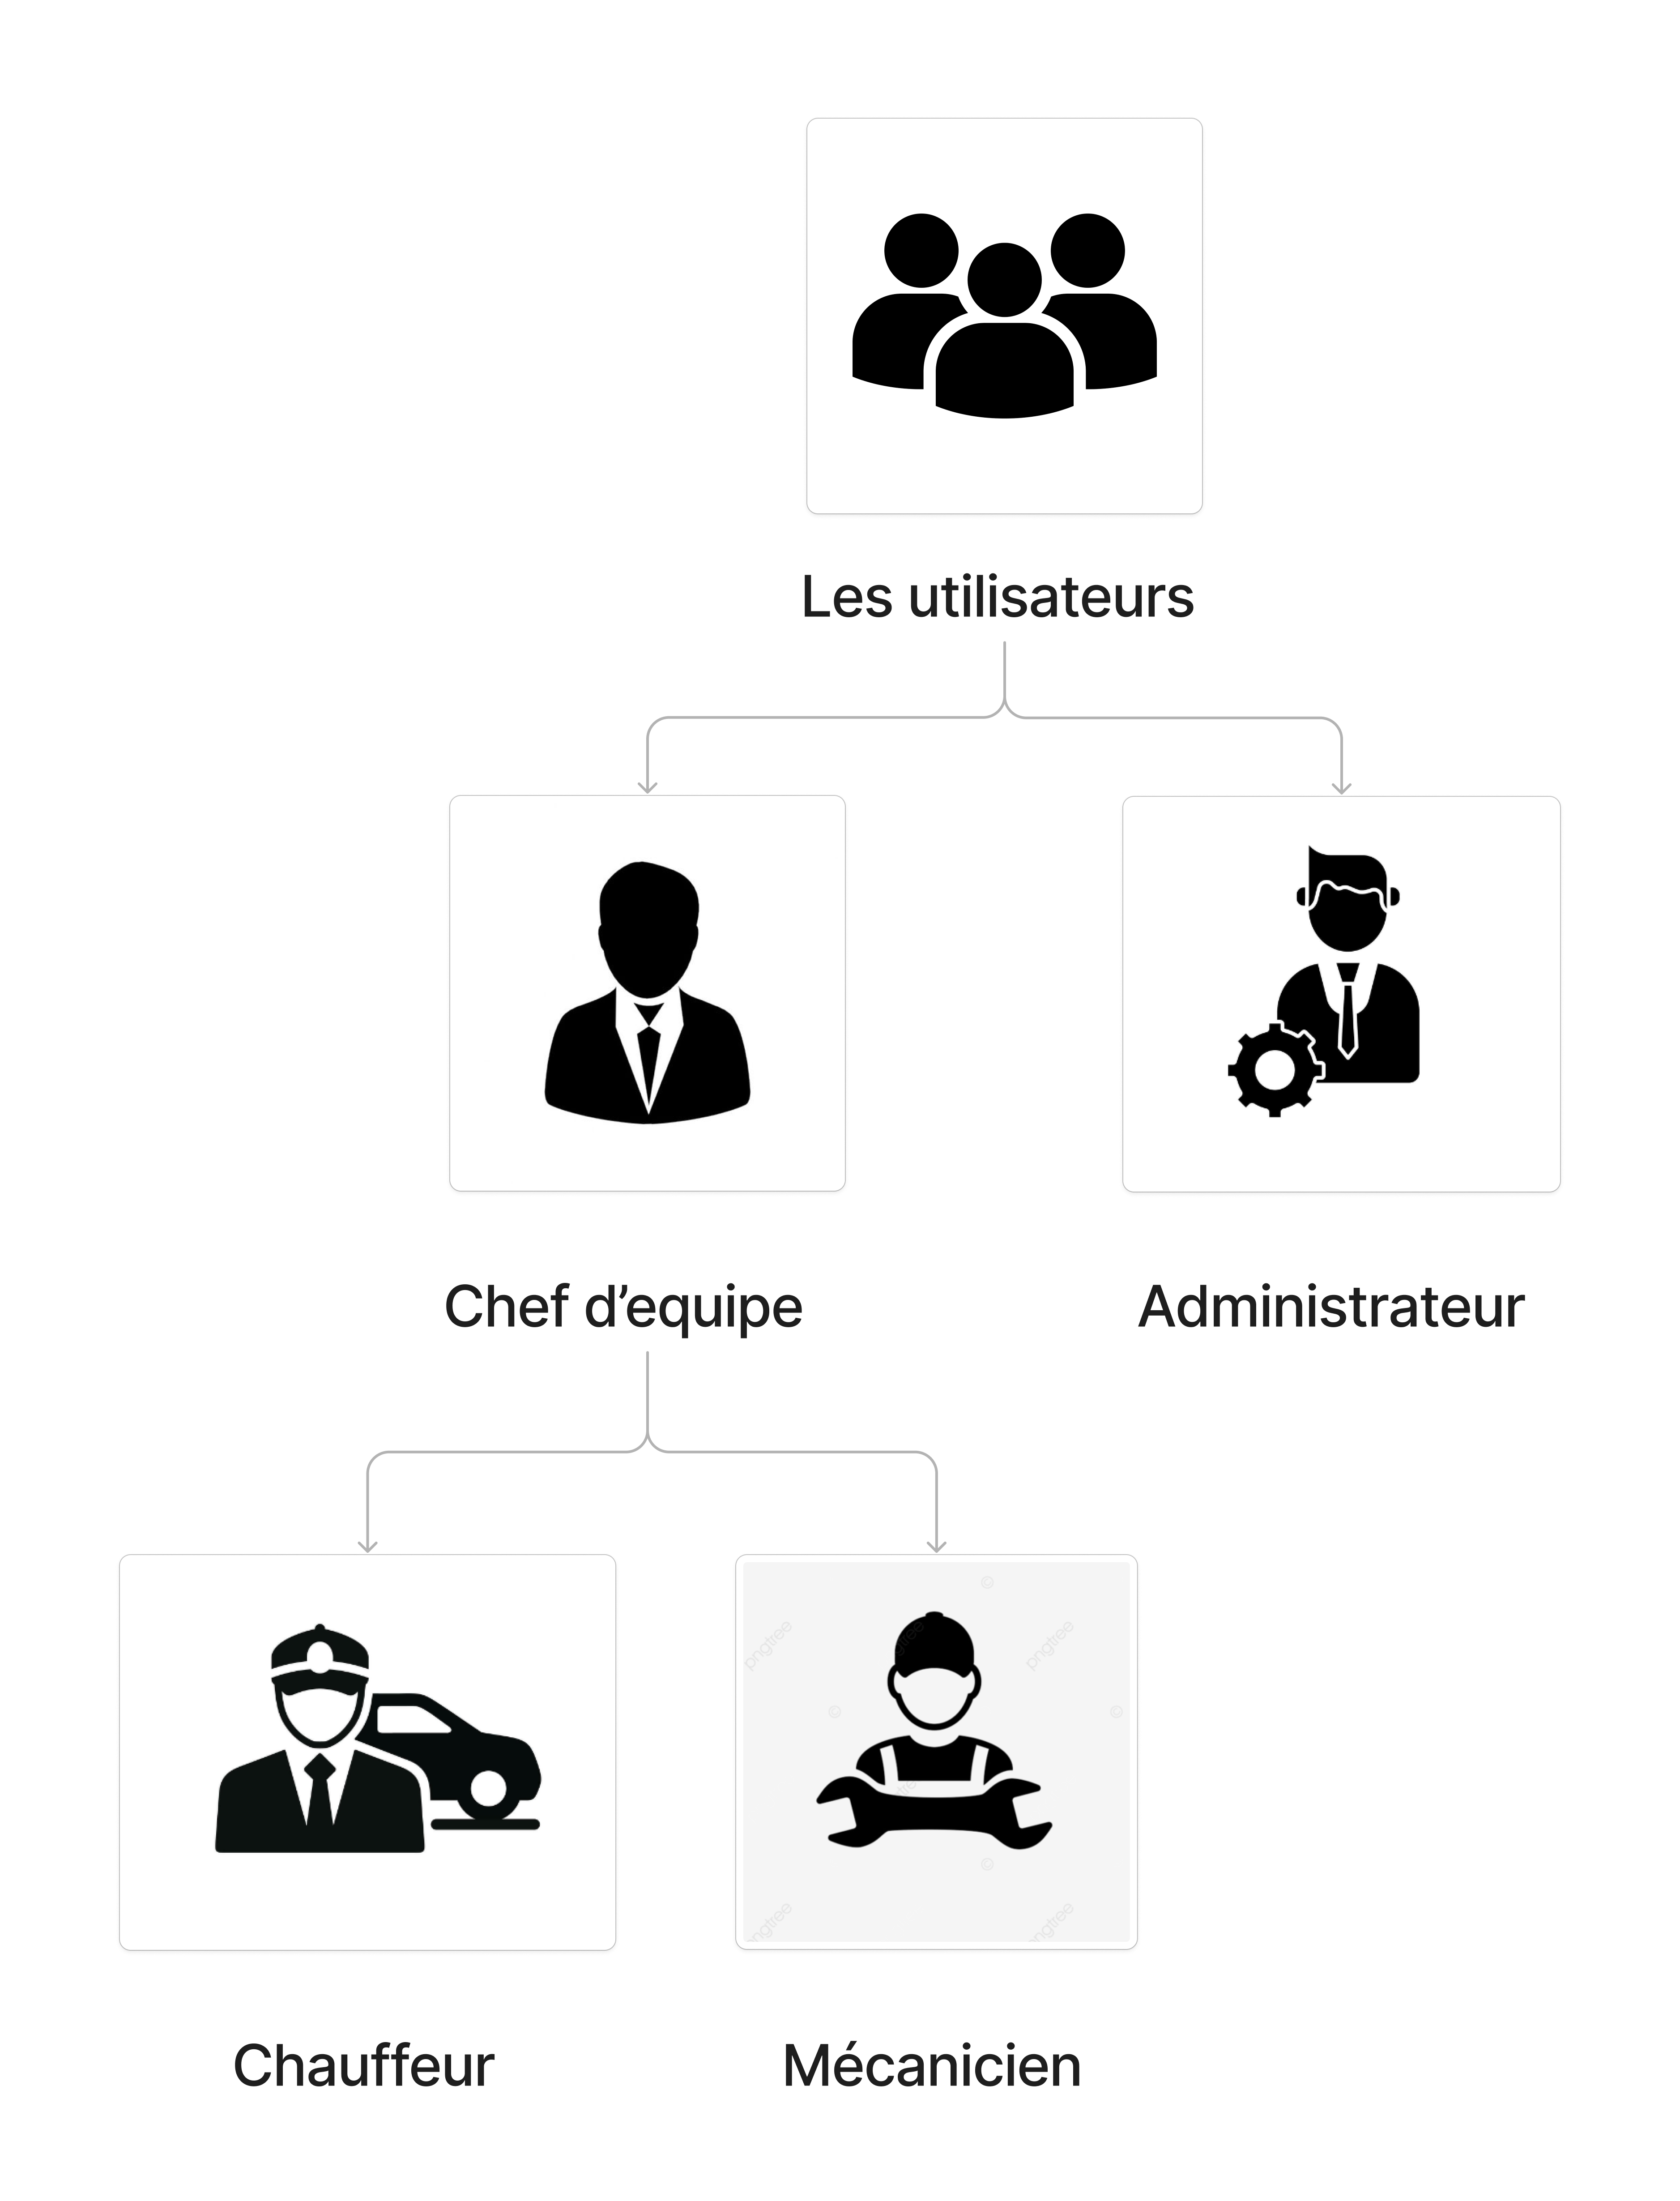
\includegraphics[width=0.7\textwidth,height=12cm]{chap2.images/Diagramme des acteurs.png}
  \caption{Diagramme des acteurs}
\end{figure}

%________________________________________________________________________________________________________




%__________________________________________________________________________________________________________

\newpage
\subsection{Besoins fonctionnels}
La spécification des besoins fonctionnels détermine les exigences fonctionnelles ainsi que les principaux objectifs et fonctionnalités de l'application. En d'autres termes, elle spécifie ce que le système étudié doit faire.\\

\begin{itemize}


  \item[$\bullet$] \textbf {S’authentifier:} Toute personne inscrite devra s’authentifier en saisissant son nom d’utilisateur ainsi que son mot de passe afin d’accéder aux fonctionnalités du statut sous lequelle elle est inscrite.\\

  \item[$\bullet$] \textbf {Gérer profil:} Chaque acteur qu’il soit administrateur, chef d'equipe, chauffeur ou même mécanicien peut gérer son propre compte.\\

  \item[$\bullet$] \textbf {Gestion des utilisateurs :} Permet à l’administrateur de gérer les comptes des utilisateurs de l’application, y compris la création, la modification et la suppression des comptes. Lors de la création d'un utilisateur (chef d'équipe, chauffeur ou mécanicien), un email contenant les paramètres de connexion ainsi qu'un manuel d'utilisation de l'application en PDF, adapté à chaque type d'utilisateur, sera envoyé automatiquement.\\

  \item[$\bullet$] \textbf {Gestion des rôles :}  Permet à l'administrateur d'attribuer des rôles spécifiques à chaque utilisateur, déterminant ainsi leurs permissions et leurs accès au système.\\

  \item[$\bullet$] \textbf {Gestion des Véhicules :} L'administrateur peut ajouter de nouveaux véhicules, supprimer des véhicules existants et visualiser la liste complète des véhicules dans le système .\\

  \item[$\bullet$] \textbf {Notifications :} Les notifications sont catégorisées (accidents, maintenance, demande de pièce ...) pour une gestion proactive des événements.\\

  \item[$\bullet$] \textbf {Création des tâches :} Permet à l'administrateur de créer, attribuer, suivre et gérer les tâches assignées aux chauffeurs, mécaniciens et chefs d'équipe. \\

  \item[$\bullet$] \textbf {Suivi des tâches :} Permet au chef d'équipe de suivre l'état et la progression des tâches assignées à son équipe, en vérifiant leur avancement et en s'assurant de leur complétion.\\

  \item[$\bullet$] \textbf {Surveillance en temps réel des déplacements des véhicules :} Donne au chef d'équipe la capacité de surveiller les déplacements en temps réel des véhicules de l'entreprise, afin de coordonner efficacement les opérations.\\

  \item[$\bullet$] \textbf {Consultation de checklist :} Permet au chauffeur de consulter les listes de vérification nécessaires avant de commencer un voyage ou une mission, garantissant ainsi la conformité et la sécurité .\\

  \item[$\bullet$] \textbf {Planification des voyages :} Autorise le chauffeur à planifier ses itinéraires et ses voyages à l'avance, en tenant compte des horaires, des destinations et d'autres paramètres pertinents. \\

  \item[$\bullet$] \textbf {Confirmation des tâches :} Permet au chauffeur de confirmer la réalisation des tâches qui lui sont assignées, telles que la livraison de marchandises ou la maintenance préventive des véhicules.\\

  \item[$\bullet$] \textbf {Consultation des tâches :} Donne au mécanicien la possibilité de consulter les tâches de maintenance assignées, y compris les réparations à effectuer et les inspections à réaliser..\\

  \item[$\bullet$] \textbf {Rapport :}  Permet au mécanicien de générer des rapports détaillés sur les travaux effectués, les pièces utilisées et l'état général des véhicules, contribuant ainsi à la gestion proactive de la maintenance.\\


\end{itemize}


%__________________________________________________________________________________________________________


\subsection{Besoins non fonctionnels}
La définition des besoins non fonctionnels est cruciale pour déterminer les caractéristiques et la qualité requises du système. Ils n’affectent pas directement les fonctionnalités de l'application, mais peuvent avoir un impact sur sa performance et son efficacité globale. Il est important de ne pas les négliger lors de la conception et du développement de l'application. Les principaux besoins non fonctionnels de cette application sont:

\begin{itemize}
  \item[$\bullet$] \textbf {Simplicité d'utilisation}:  Assurer une interface utilisateur intuitive et conviviale pour toutes les catégories d'utilisateurs, minimisant ainsi la courbe d'apprentissage et favorisant l'adoption de l'application.\\

  \item[$\bullet$] \textbf {Sécurité des données}: Assurer la confidentialité, l'intégrité et la disponibilité des données sensibles telles que les informations sur les véhicules, les tâches et les utilisateurs.\\

  \item[$\bullet$] \textbf {Évolutivité}: Concevoir l'application pour qu'elle puisse s'adapter à l'augmentation du nombre d'utilisateurs, de véhicules et de fonctionnalités sans compromettre les performances ou la fiabilité du système.\\

  \item[$\bullet$] \textbf {Disponibilité}:  Assurer la disponibilité continue de l'application, minimisant ainsi les temps d'arrêt et les interruptions des opérations.


\end{itemize}


%__________________________________________________________________________________________________________


\newpage
\subsection{Diagramme de cas d'utilisation}
La figure 2.2 illustre le diagramme de cas d'utilisation géneral de notre application.
\begin{figure}[ht]
  \centering
  \includegraphics[width=1\textwidth,height=18cm]{chap2.images/use case global.png}
  \caption{Diagramme de cas d'utilisation global}
\end{figure}



%__________________________________________________________________________________________________________



\newpage
\section{Pilotage du projet avec Scrum}
Cette section comportant l’équipe du projet et ses rôles, le backlog du produit et le découpage du projet en sprint, présente le pilotage du projet avec Scrum .
\subsection{Équipe et rôles}
L'équipe responsable du pilotage du projet est composée de:\\
\begin{itemize}
  \item[$\bullet$]\textbf{Product owner: } Digital Identity.\\
  \item[$\bullet$]\textbf{Scrum master: } C'est un membre de l'équipe de développement de Digid Mr Baha jaouane . \\
  \item[$\bullet$]\textbf{Scrum team: }C'est l'équipe de développement qui englobe nous mêmes Mimouni med aziz  et Balti firas. \\
\end{itemize}
\subsection{Contraintes et exigences}
La réussite du développement et de l'implémentation d'une solution technique dépend de l'identification des besoins réels des parties prenantes. Certaines fonctionnalités et besoins sont plus importants que d'autres, et il est crucial de les réaliser en premier pour assurer la continuité et la clarté de l'application. Pour cela, il est essentiel d'établir un ordre de priorité afin de coordonner les tâches à effectuer. Ce processus implique de classer les besoins en trois catégories selon leur importance : élevée, moyenne et faible, tout au long du cycle de vie de la solution technique.
\subsection{Risques}
Les principaux obstacles qui peuvent entraver notre progression sont la complexité de l'application et les exigences à respecter. Il est également important de prendre en compte la représentation des fonctionnalités similaires au cours de deux sprints consécutifs, afin d'éviter toute redondance inutile. Pour minimiser les risques, il est donc préférable de regrouper ces fonctionnalités similaires ensemble, plutôt que de les aborder séparément.
\subsection{Backlog du produit}
Le backlog du produit (Table 2.1) montre la liste des exigences et des fonctionnalités qui doivent être réalisées pour un produit donné ainsi que leurs degrés de priorité et de risque. Il sert de document de référence pour l'équipe de développement, les parties prenantes et les clients, afin de s'assurer que les travaux sont bien alignés sur les objectifs du projet et les besoins des utilisateurs finaux.



%______________________________________________________________________________________________________







\begin{table}[htbp]
  \centering
  \renewcommand{\arraystretch}{4.15} % Facteur d'étirement des lignes
  \begin{tabular}{|c|c|c|c|}
    \hline
    \textbf{ID}   & \textbf{USER STORIES}                                                                                                                                                            & \textbf{PRIORITE} & \textbf{RISQUE} \\

    %%%%%%%%%%%%%%%%%%%%%%%%%%%%%%%%%%%%%%%%%%%%%%%%%%%%%%%%%%%%%%        

    \hline
    \textbf{US1}  & \parbox{9cm}{\centering En tant qu’administrateur,, chauffeur, chef d'équipe et mécanicien je veux m'authentifier pour que j'accède a mon espace.}                               & Elevée            & Faible          \\
    \hline
    \textbf{US2}  & \parbox{9cm}{\centering En tant qu’administrateur,, chauffeur, chef d'équipe et mécanicien je veux me déconnecter pour que je quitte l'application.}                             & Elevée            & Faible          \\
    \hline
    \textbf{US3}  & \parbox{9cm}{\centering En tant qu’administrateur,, chauffeur, chef d'équipe et mécanicien je veux modifier mon profil.}                                                         & Elevée            & Faible          \\
    \hline
    \textbf{US4}  & \parbox{9cm}{\centering En tant qu'administrateur, je veux pouvoir gérer les rôles des utilisateurs, afin de contrôler l'accès aux fonctionnalités de l'application}             & Elevée            & Faible          \\
    \hline
    \textbf{US5}  & \parbox{9cm}{\centering En tant qu'administrateur, je veux ajouter, supprimer et  visualiser les véhicules .}                                                                    & Elevée            & Faible          \\
    \hline
    \textbf{US6}  & \parbox{9cm}{\centering En tant qu’administrateur, je veux Gérer les utilisateurs pour que je puisse ajouter/modifier/supprimer des utilisateurs. }                              & Elevée            & Faible          \\


    %%%%%%%%%%%%%%%%%%%%%%%%%%%%%%%%%%%%%%%%%%%%%%%%%%%%%%%%%%%%%%

    \hline
    \textbf{US7}  & \parbox{9cm}{\centering En tant que Chef d'équipe je veux suivre le progrès et la localisation des voiture .}                                                                    & Elevée            & Faible          \\
    \hline
    \textbf{US8}  & \parbox{9cm}{\centering En tant que Chef d'équipe je veux Créer des taches pour les chauffeurs et les mécanicien .}                                                              & Elevée            & Faible          \\
    \hline
    \textbf{US9}  & \parbox{9cm}{\centering En tant que Mécanicien je veux Consulter les détails des interventions .}                                                                                & Elevée            & Faible          \\
    \hline
    \textbf{US10} & \parbox{9cm}{\centering En tant que Chauffeur je veux consulter la checklist avant et aprés le départ . }                                                                        & Elevée            & Faible          \\

    %%%%%%%%%%%%%%%%%%%%%%%%%%%%%%%%%%%%%%%%%%%%%%%%%%%%%%%%%%%%%%

    \hline
    \textbf{US11} & \parbox{9cm}{\centering En tant qu’administrateur, chauffeur, mécanicien ou chef d’équipe, je veux recevoir des notifications pour être informé en temps réel des mises à jour.} & Elevée            & Faible          \\
    \hline
  \end{tabular}
\end{table}




%%%%%%%%%%%%%%%%%%%%%%%%%%%%%%%%%%%%%%%%%%%%%%%%%%%%%%%%%%%%%%
\begin{table}[htbp]
  \centering
  \renewcommand{\arraystretch}{4.15} % Facteur d'étirement des lignes
  \begin{tabular}{|c|c|c|c|}

    \hline
    \textbf{US12} & \parbox{11cm}{\centering En tant que Mécanicien je veux Générer des rapports pour que je puisse documenter les détails de chaque intervention.}                                       & Elevée & Faible \\
    \hline
    \textbf{US13} & \parbox{11cm}{\centering En tant qu’administrateur, je veux avoir accès à un tableau de bord pour que je puisse superviser l'ensemble des opérations.}                                & Elevée & Faible \\
    \hline
    \textbf{US14} & \parbox{11cm}{\centering En tant que Chef d'équipe, je veux un tableau de bord pour suivre les déplacements en temps réel des chauffeurs et gérer les missions de manière proactive.} & Elevée & Faible \\
    \hline
    \textbf{US15} & \parbox{11cm}{\centering En tant que Chauffeur je veux Consulter un tableau de bord pour que je puisse avoir une vue claire de mes missions actuelles}                                & Elevée & Faible \\
    \hline
    \textbf{US16} & \parbox{11cm}{\centering En tant que Mécanicien, je veux consulter un tableau de bord pour avoir une vue d'ensemble des opérations de maintenance.}                                   & Elevée & Faible \\
    \hline
  \end{tabular}
  \bigskip
  \caption{Backlog du produit}
  \label{tab:my_label}
\end{table}




%______________________________________________________________________________________________


\newpage{}
\section{Conception de l'application}

Dans cette section, nous présentons les prototypes de l'applications , la charte graphique, le plan de l'application ainsi que le diagramme de classes du domaine et le diagramme de gantt.

\subsection{Prototypes de l'application}


Les figure 2.3 et 2.4 illustrent les ecrans de chargement dans l'application.

\begin{figure}[h!]
  \centering
  \begin{minipage}[t]{0.60\textwidth}
    \centering
    
\includegraphics[width=1\textwidth, height=6cm]{chap2.images/splash web.png}
    \caption{Ecran de chargement - Web}
  \end{minipage}
  \hfill
  \begin{minipage}[t]{0.38\textwidth}
    \centering
    
\includegraphics[width=0.6\textwidth, height=6cm]{chap2.images/splash mob.png}
    \caption{\centering{Ecran de chargement - Mobile}}
  \end{minipage}
\end{figure}


\newpage
Les figure 2.5 et 2.6 illustrent les  pages permettant a l'utilisateur de s'authentifier dans l'application.

\begin{figure}[h!]
  \centering
  \begin{minipage}[t]{0.60\textwidth}
    \centering
    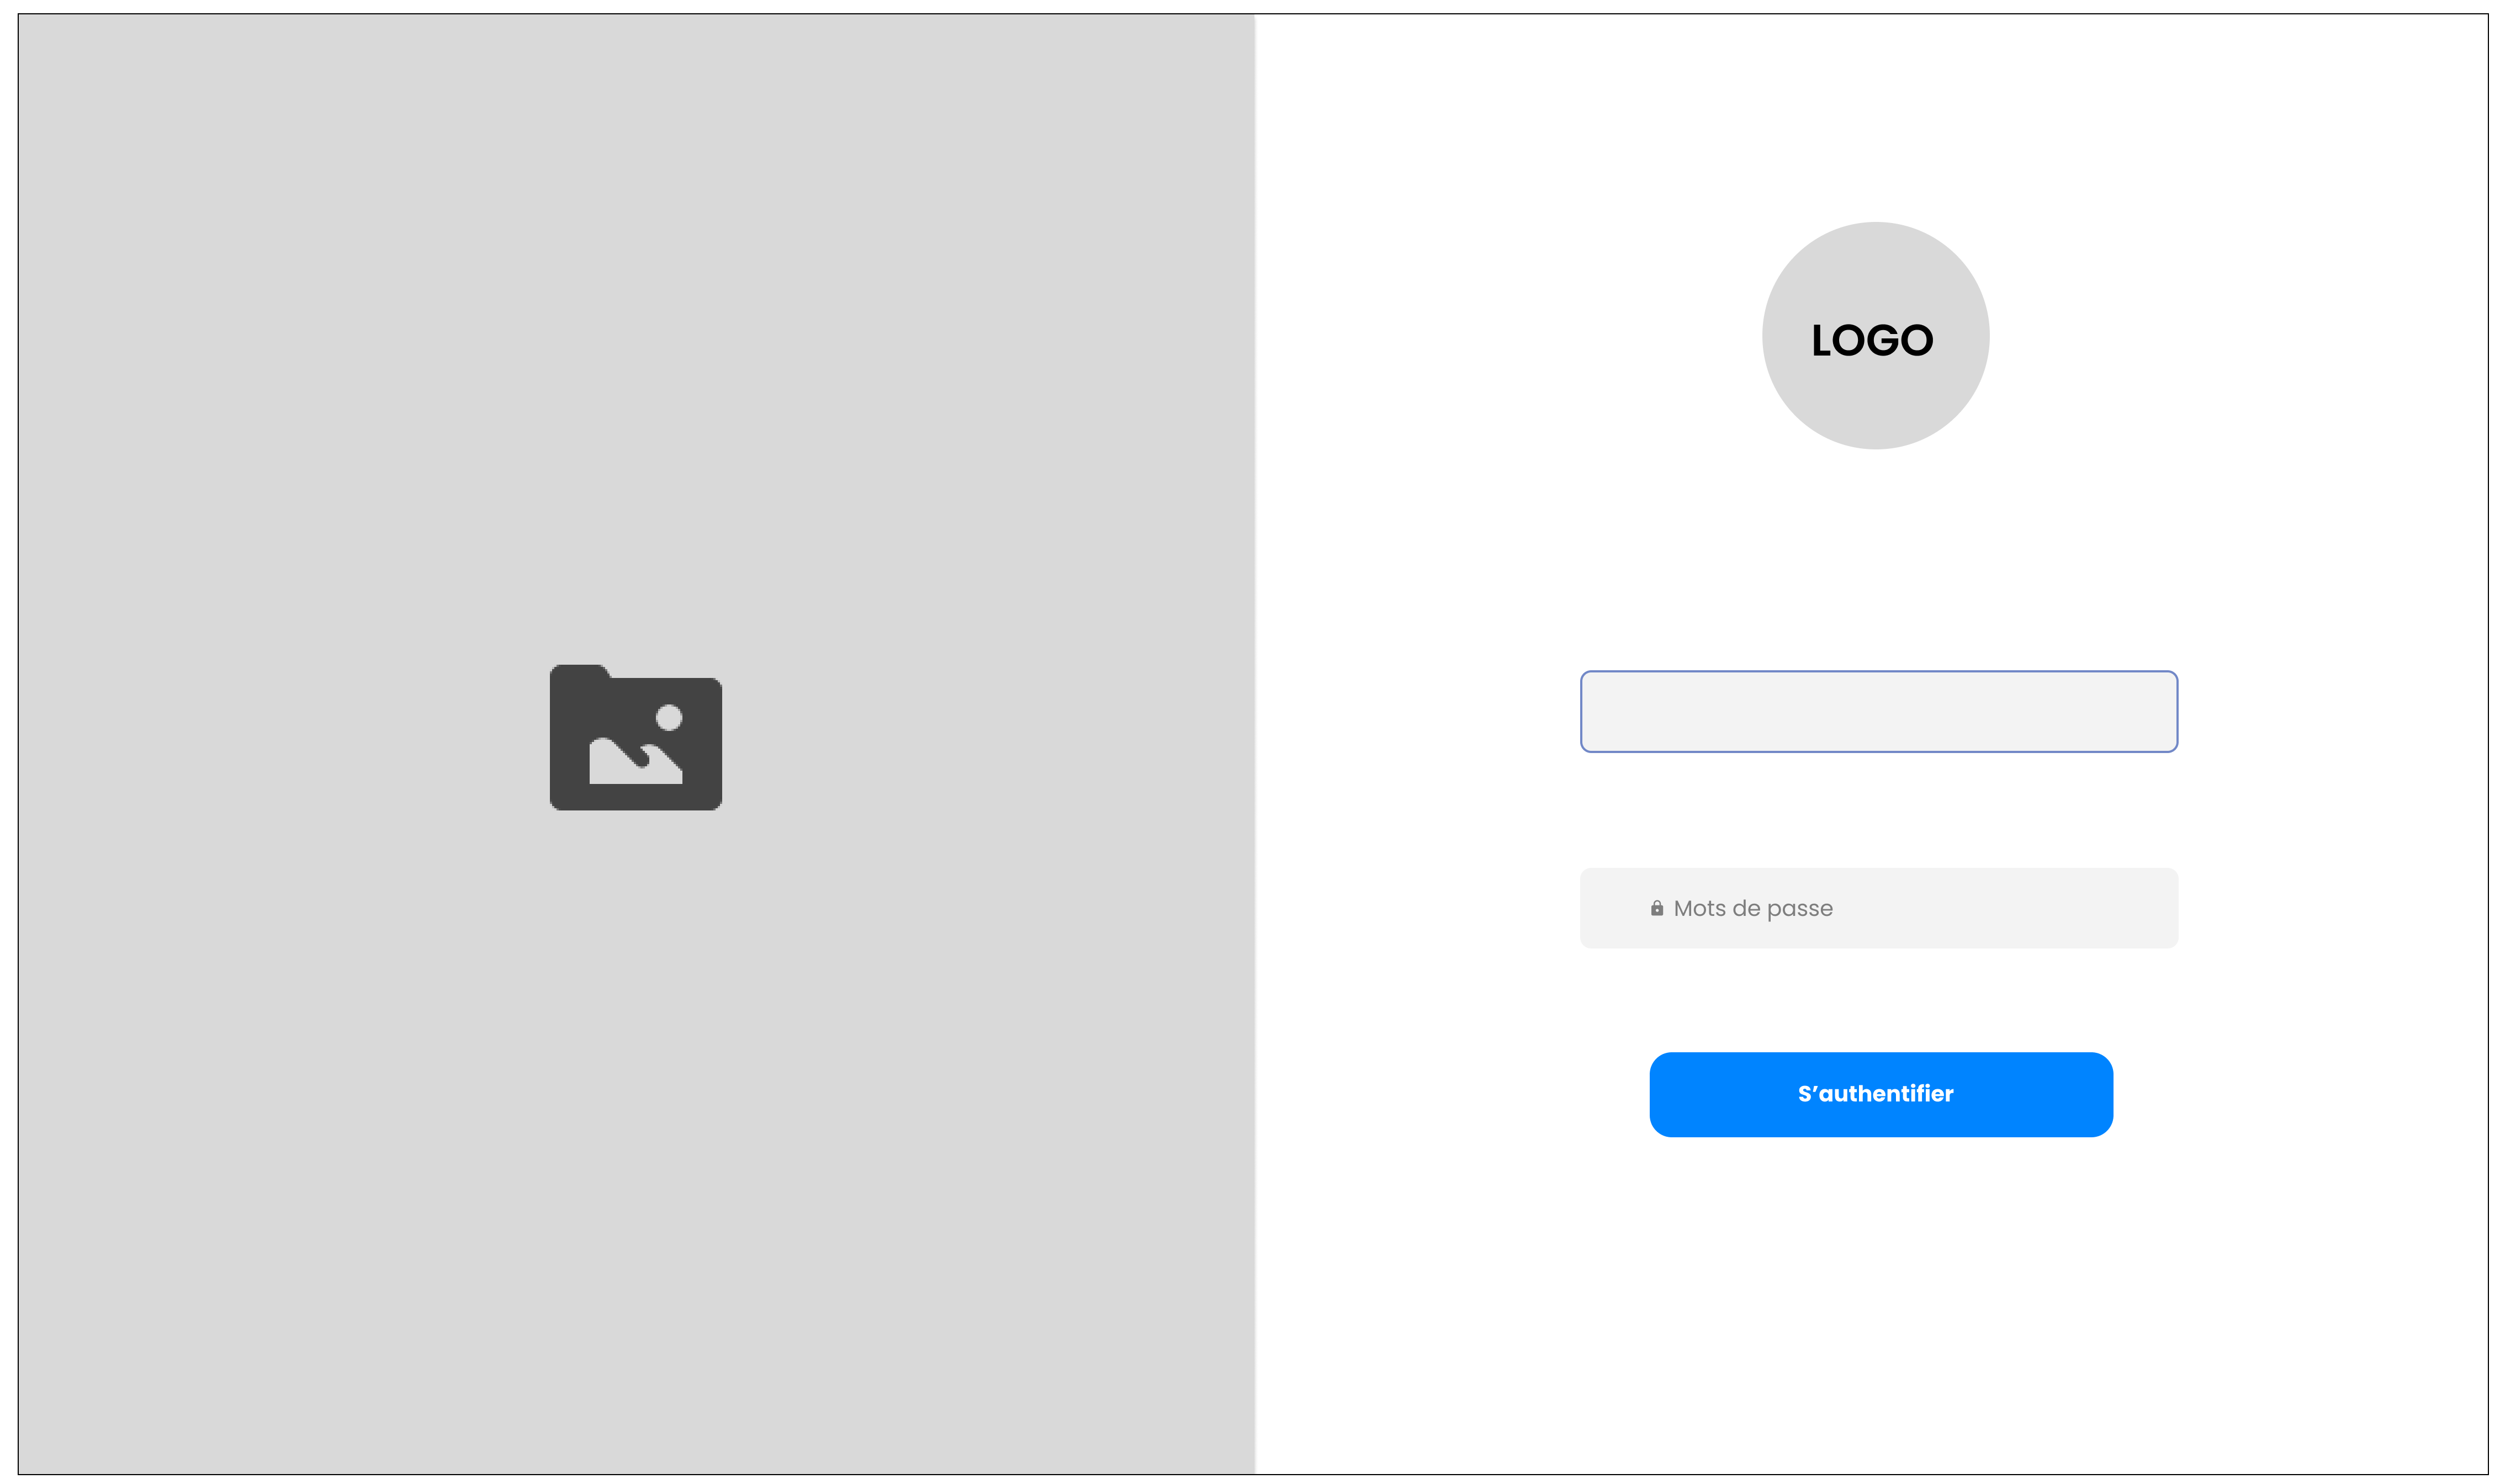
\includegraphics[width=1\textwidth, height=6cm]{chap2.images/prot authentification.png}
    \caption{Interface d'authentification - Web}
  \end{minipage}
  \hfill
  \begin{minipage}[t]{0.38\textwidth}
    \centering
    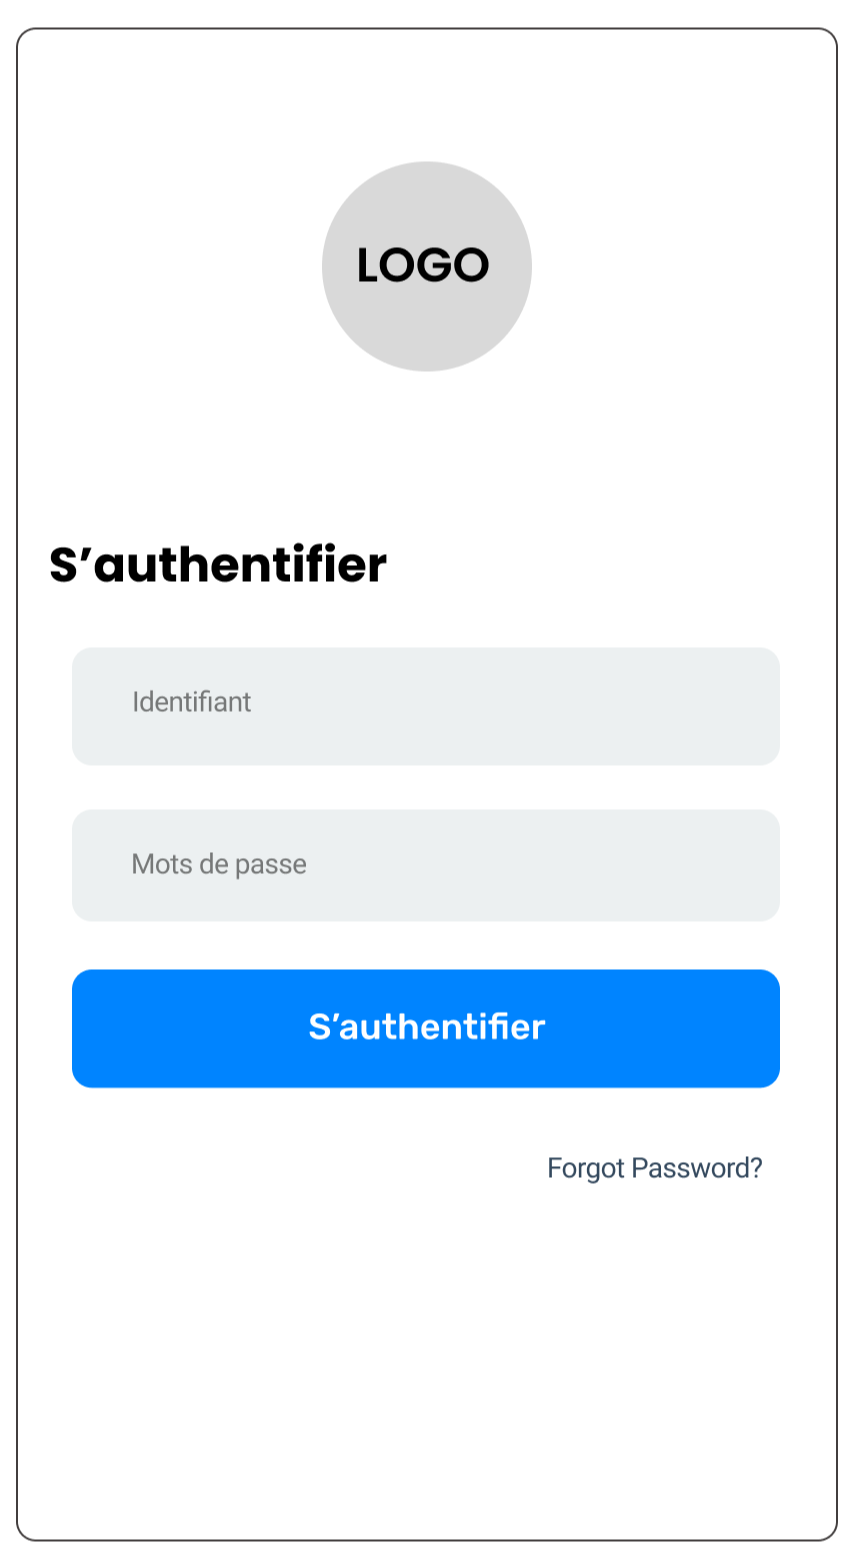
\includegraphics[width=0.6\textwidth, height=6cm]{chap2.images/prot authentification mob.png}
    \caption{\centering{Interface d'authentification - Mobile}}
  \end{minipage}
\end{figure}

\vspace{1.2cm}

Les figure 2.7 et 2.8 illustrent les  pages permettant a l'utilisateur de modifier leur profils.

\begin{figure}[h!]
  \centering
  \begin{minipage}[t]{0.60\textwidth}
    \centering
    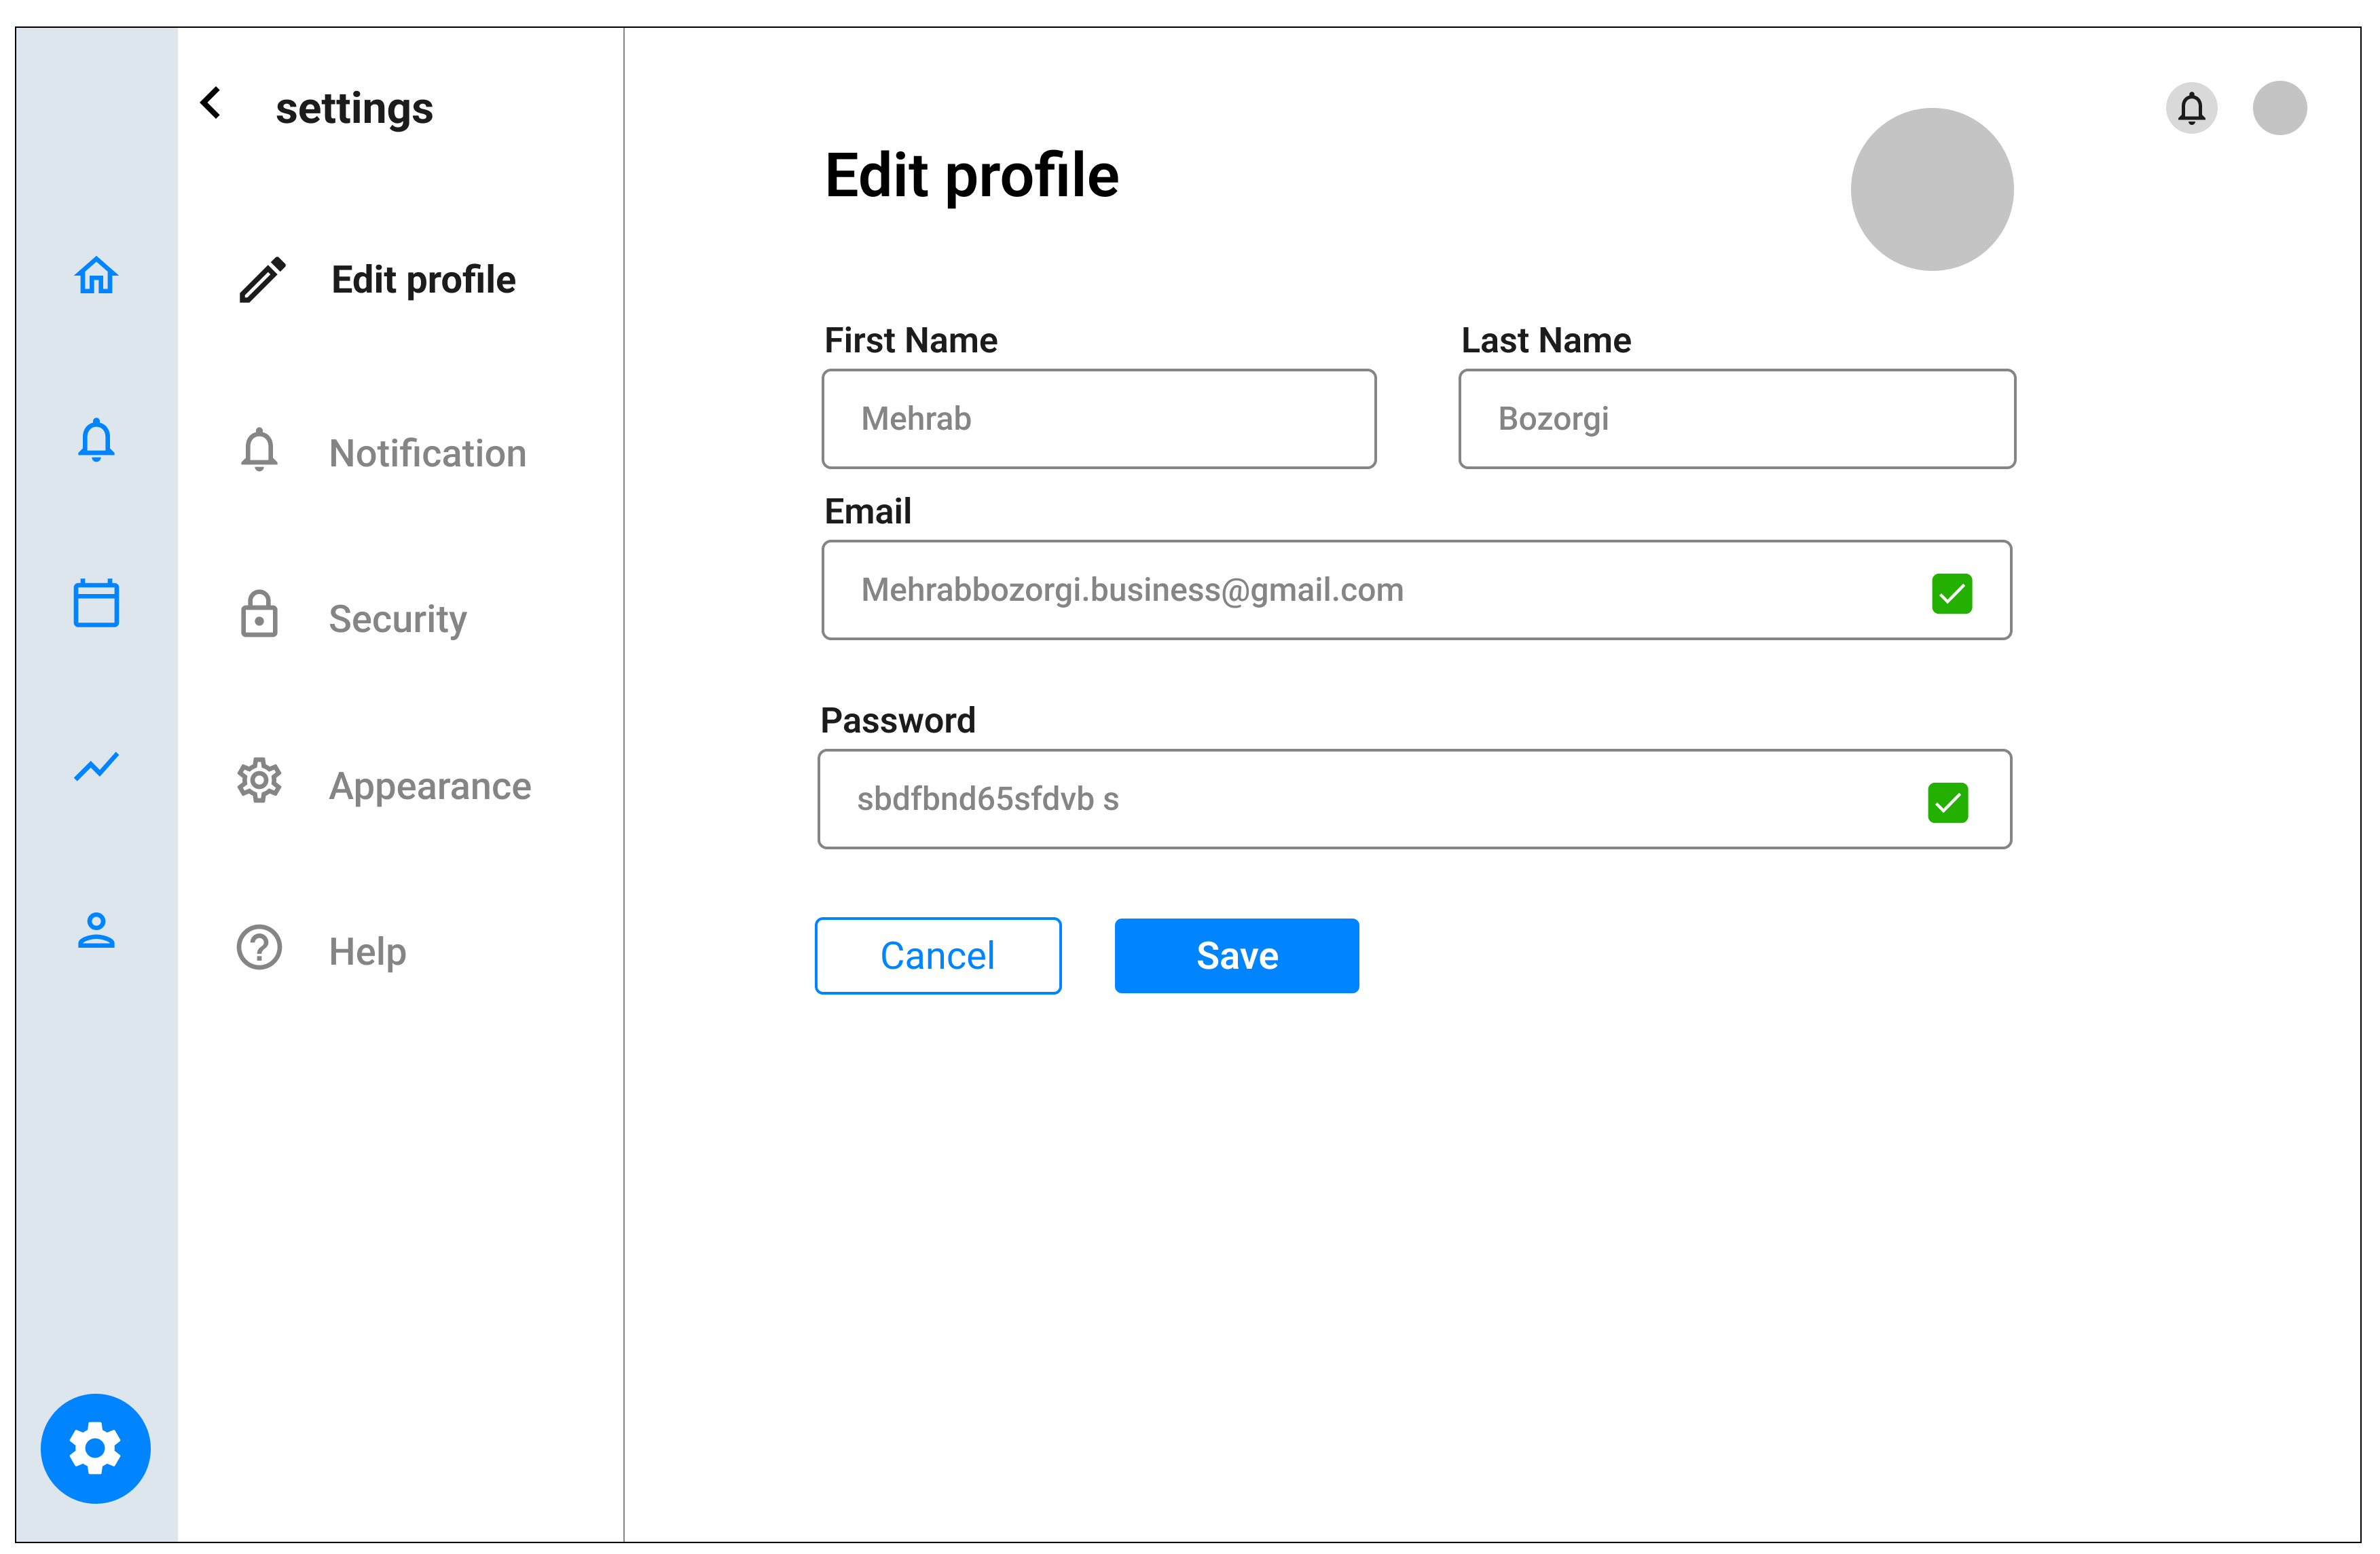
\includegraphics[width=1\textwidth, height=6cm]{chap2.images/prot modifer web.png}
    \caption{Interface de profil- Web}
  \end{minipage}
  \hfill
  \begin{minipage}[t]{0.38\textwidth}
    \centering
    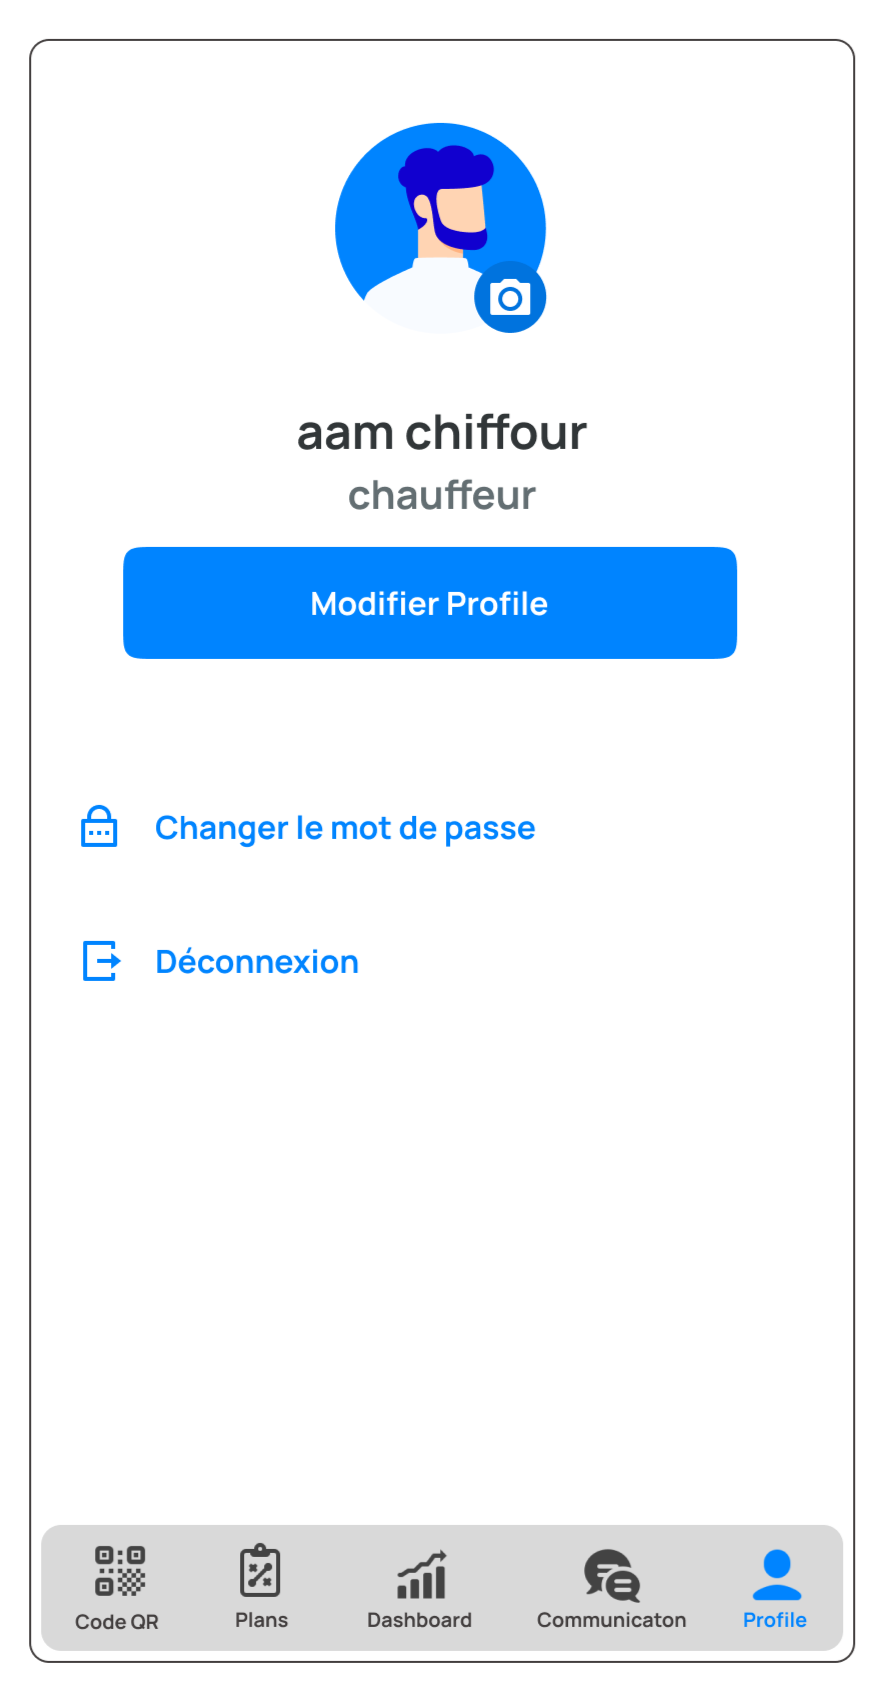
\includegraphics[width=0.6\textwidth, height=6cm]{chap2.images/prot modifier mob.png}
    \caption{\centering{Interface de profil - Mobile}}
  \end{minipage}
\end{figure}





\newpage
En plus, les figure 2.9 et 2.10 illustrent les interfaces de gestion des utilisateurs par l'administrateur.
\begin{figure}[h!]
  \centering
  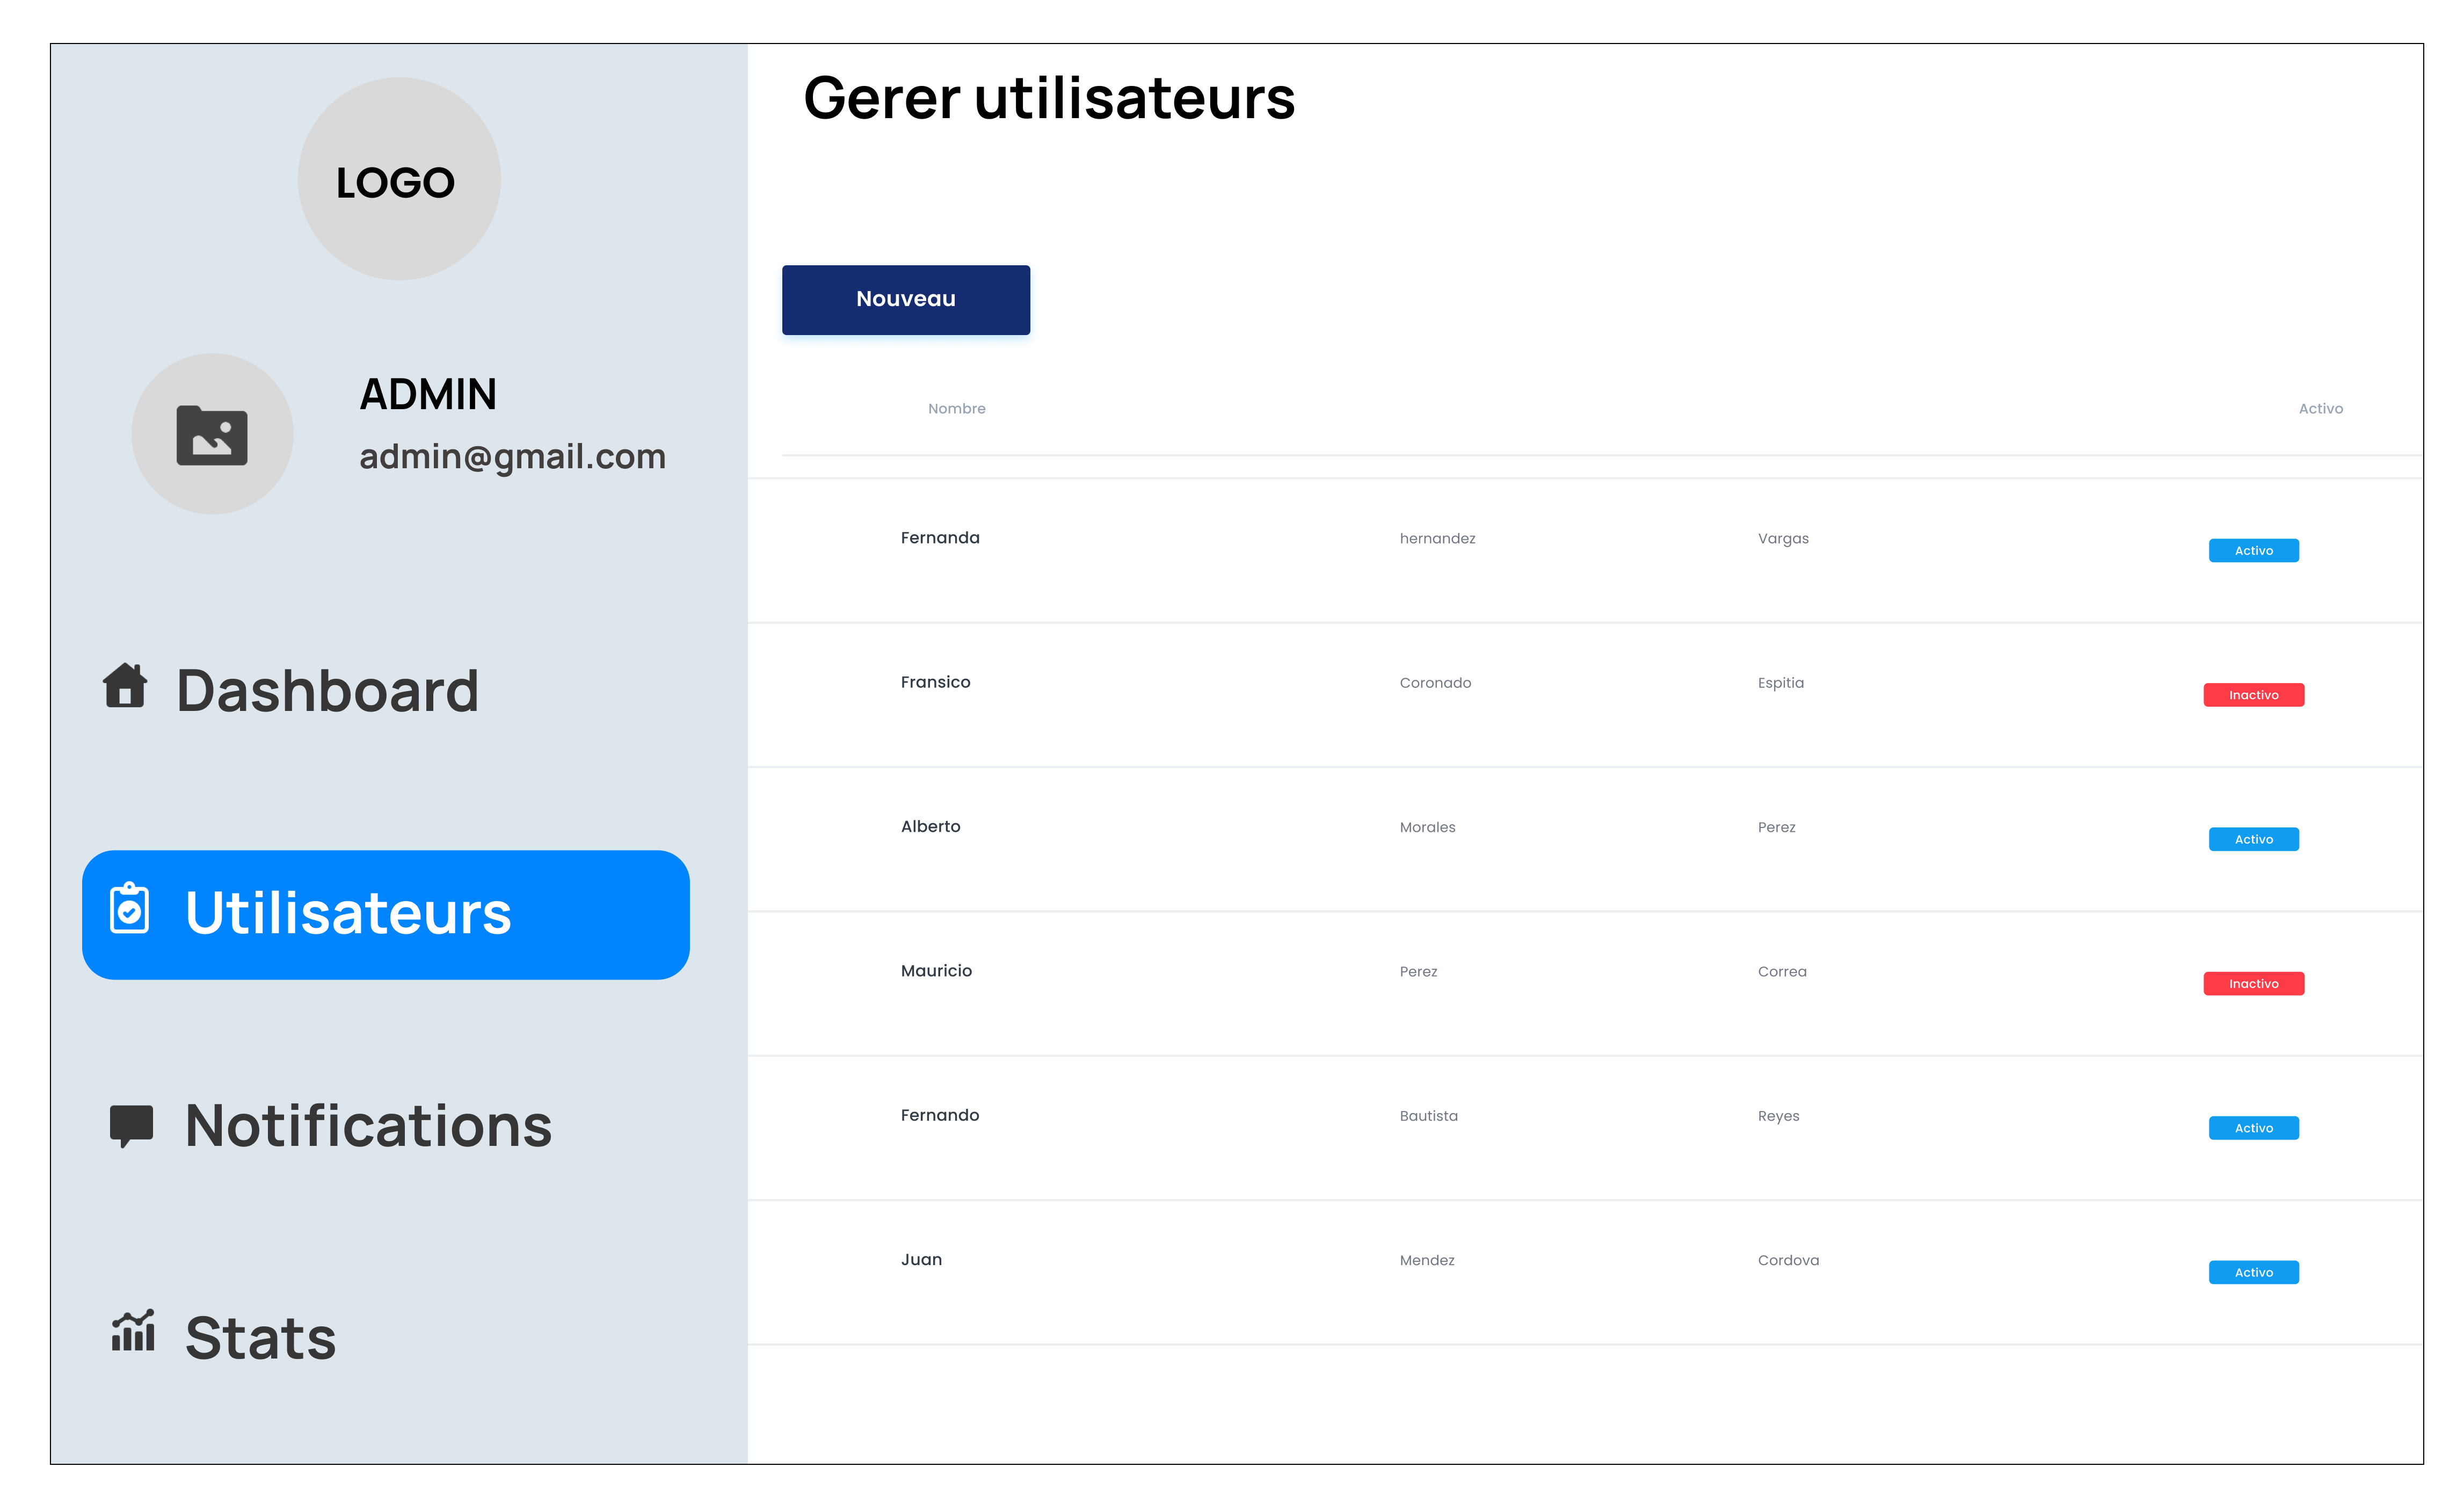
\includegraphics[width=0.9\textwidth, height=8cm]{chap2.images/prot gestion user.png}
  \caption{Interface de gestion des utilisateurs}
\end{figure}
\begin{figure}[h!]
  \centering
  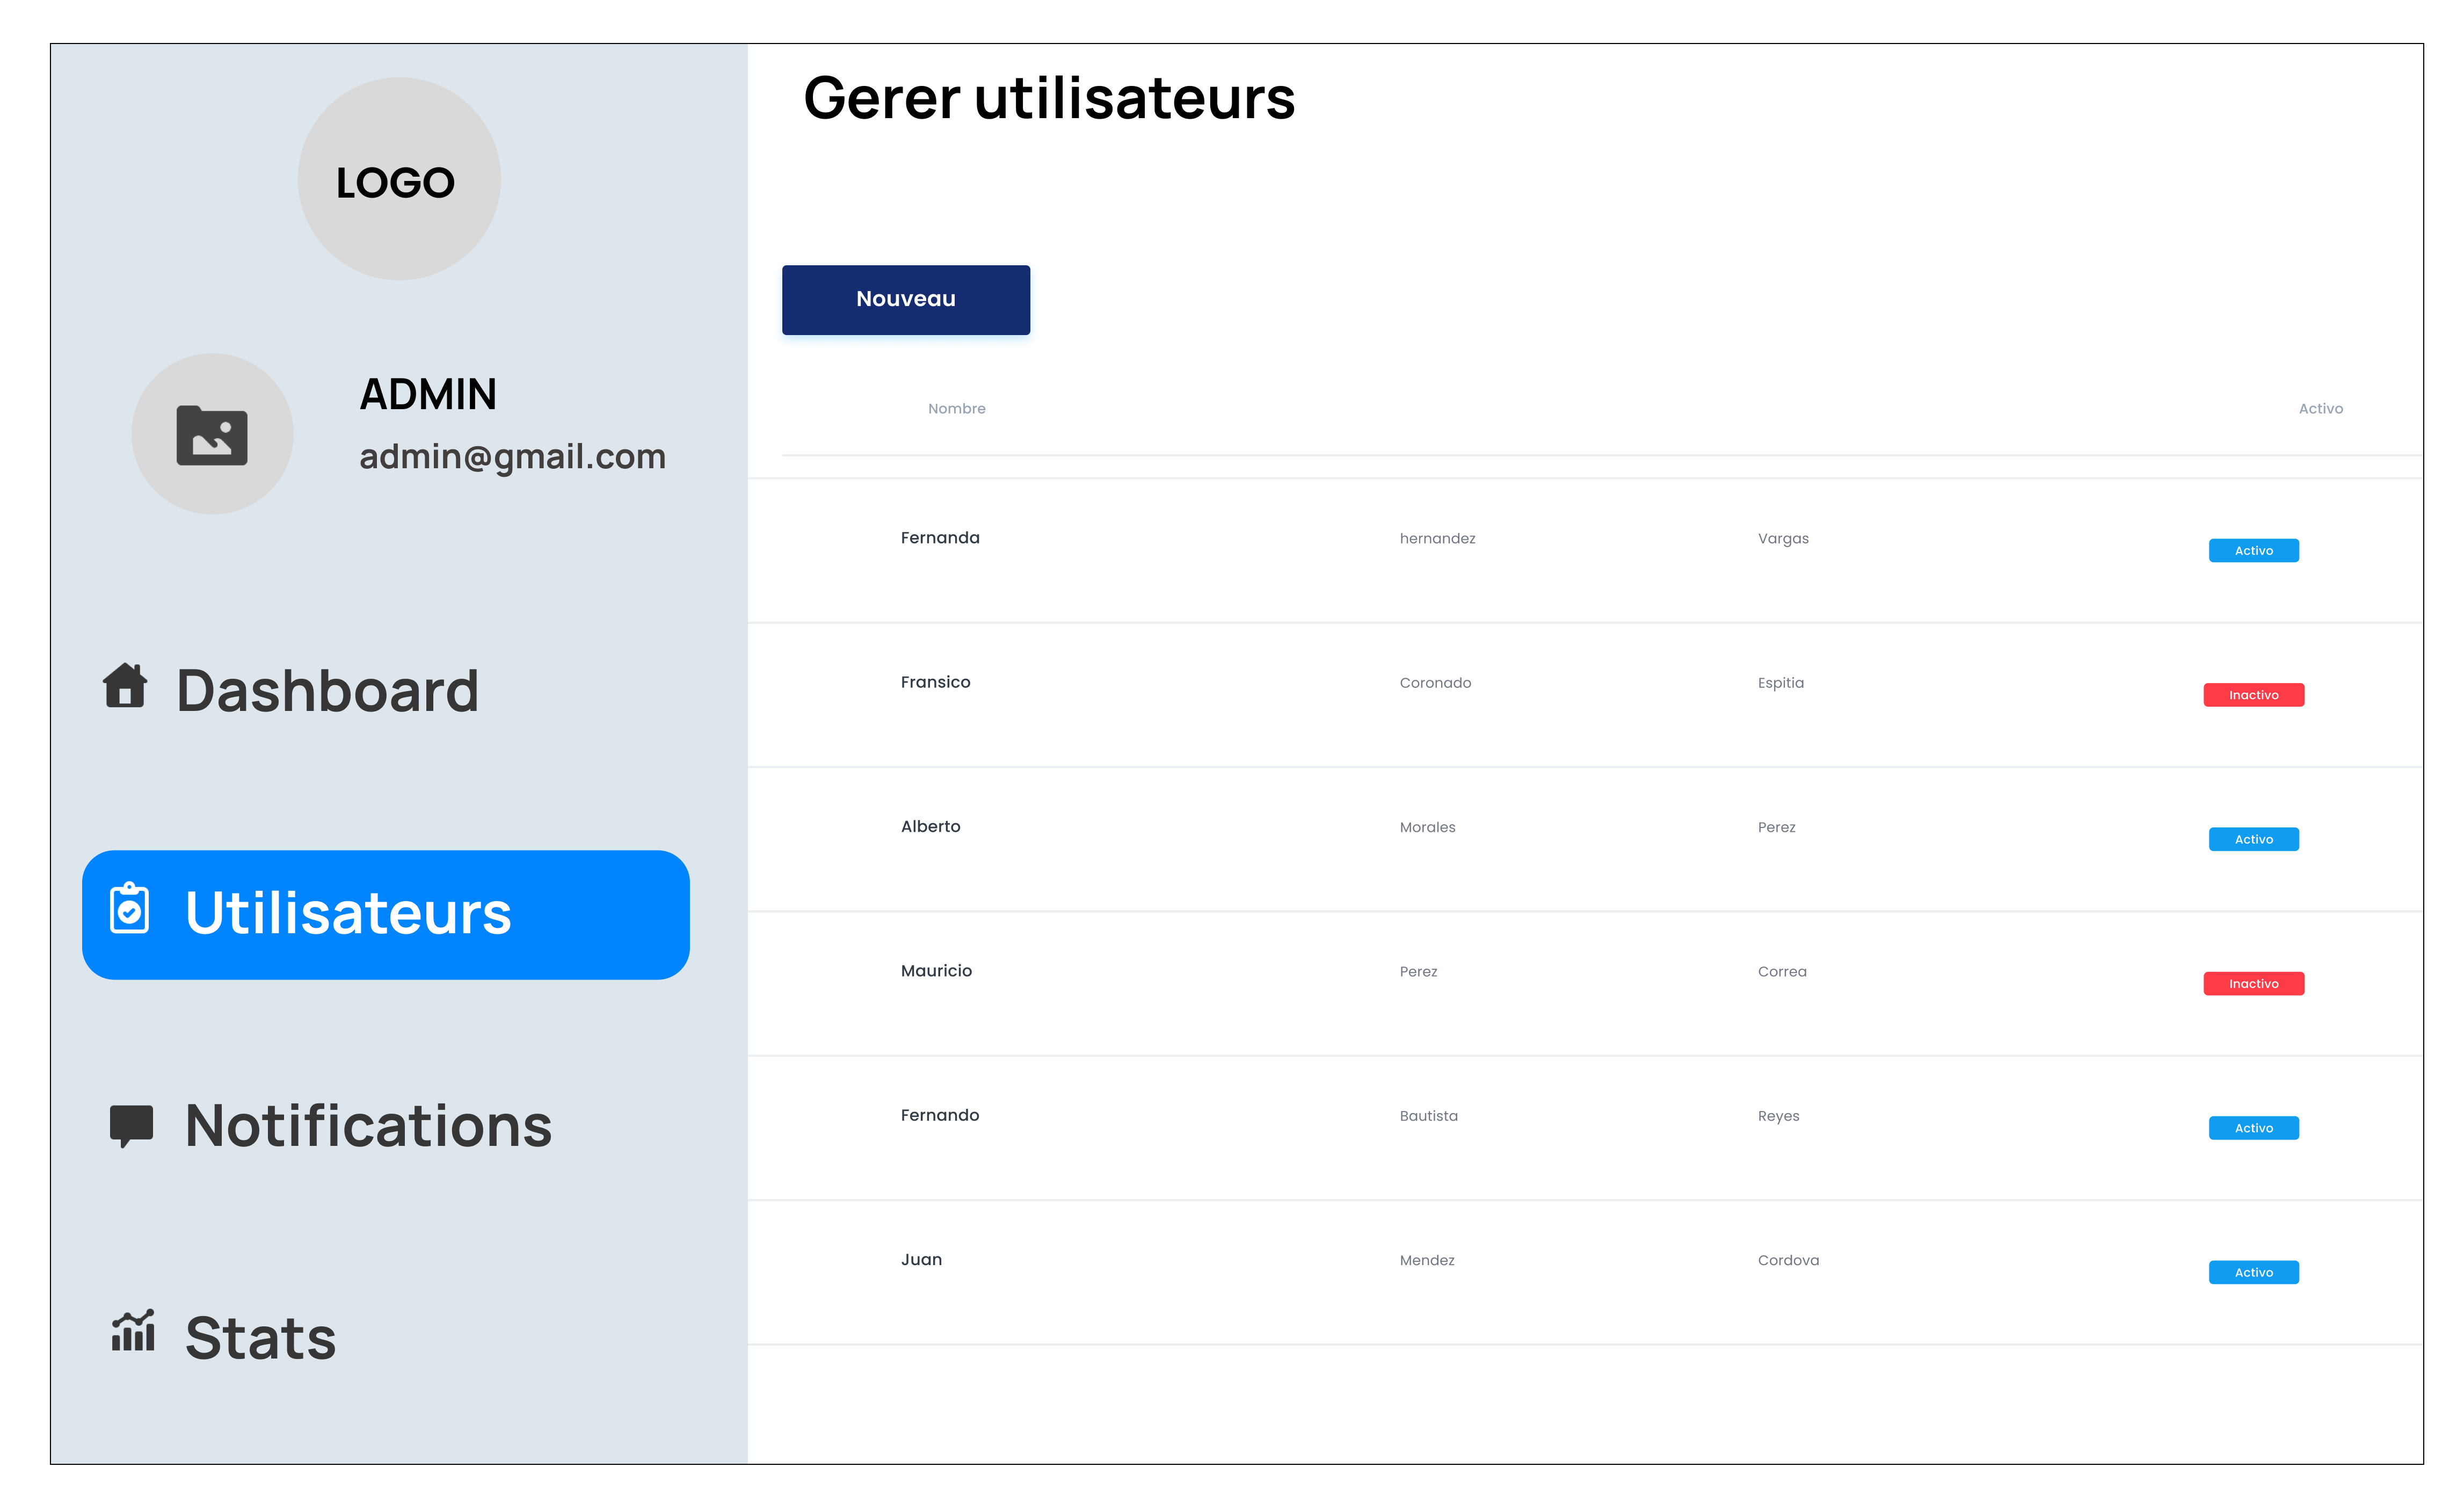
\includegraphics[width=0.9\textwidth, height=8cm]{chap2.images/prot gestion user.png}
  \caption{Interface de création d'un nouvel utilisateur}
\end{figure}

\newpage
Les figure 2.11 et 2.12 illustrent les  pages permettant ....

\begin{figure}[h!]
  \centering
  \begin{minipage}[t]{0.60\textwidth}
    \centering
    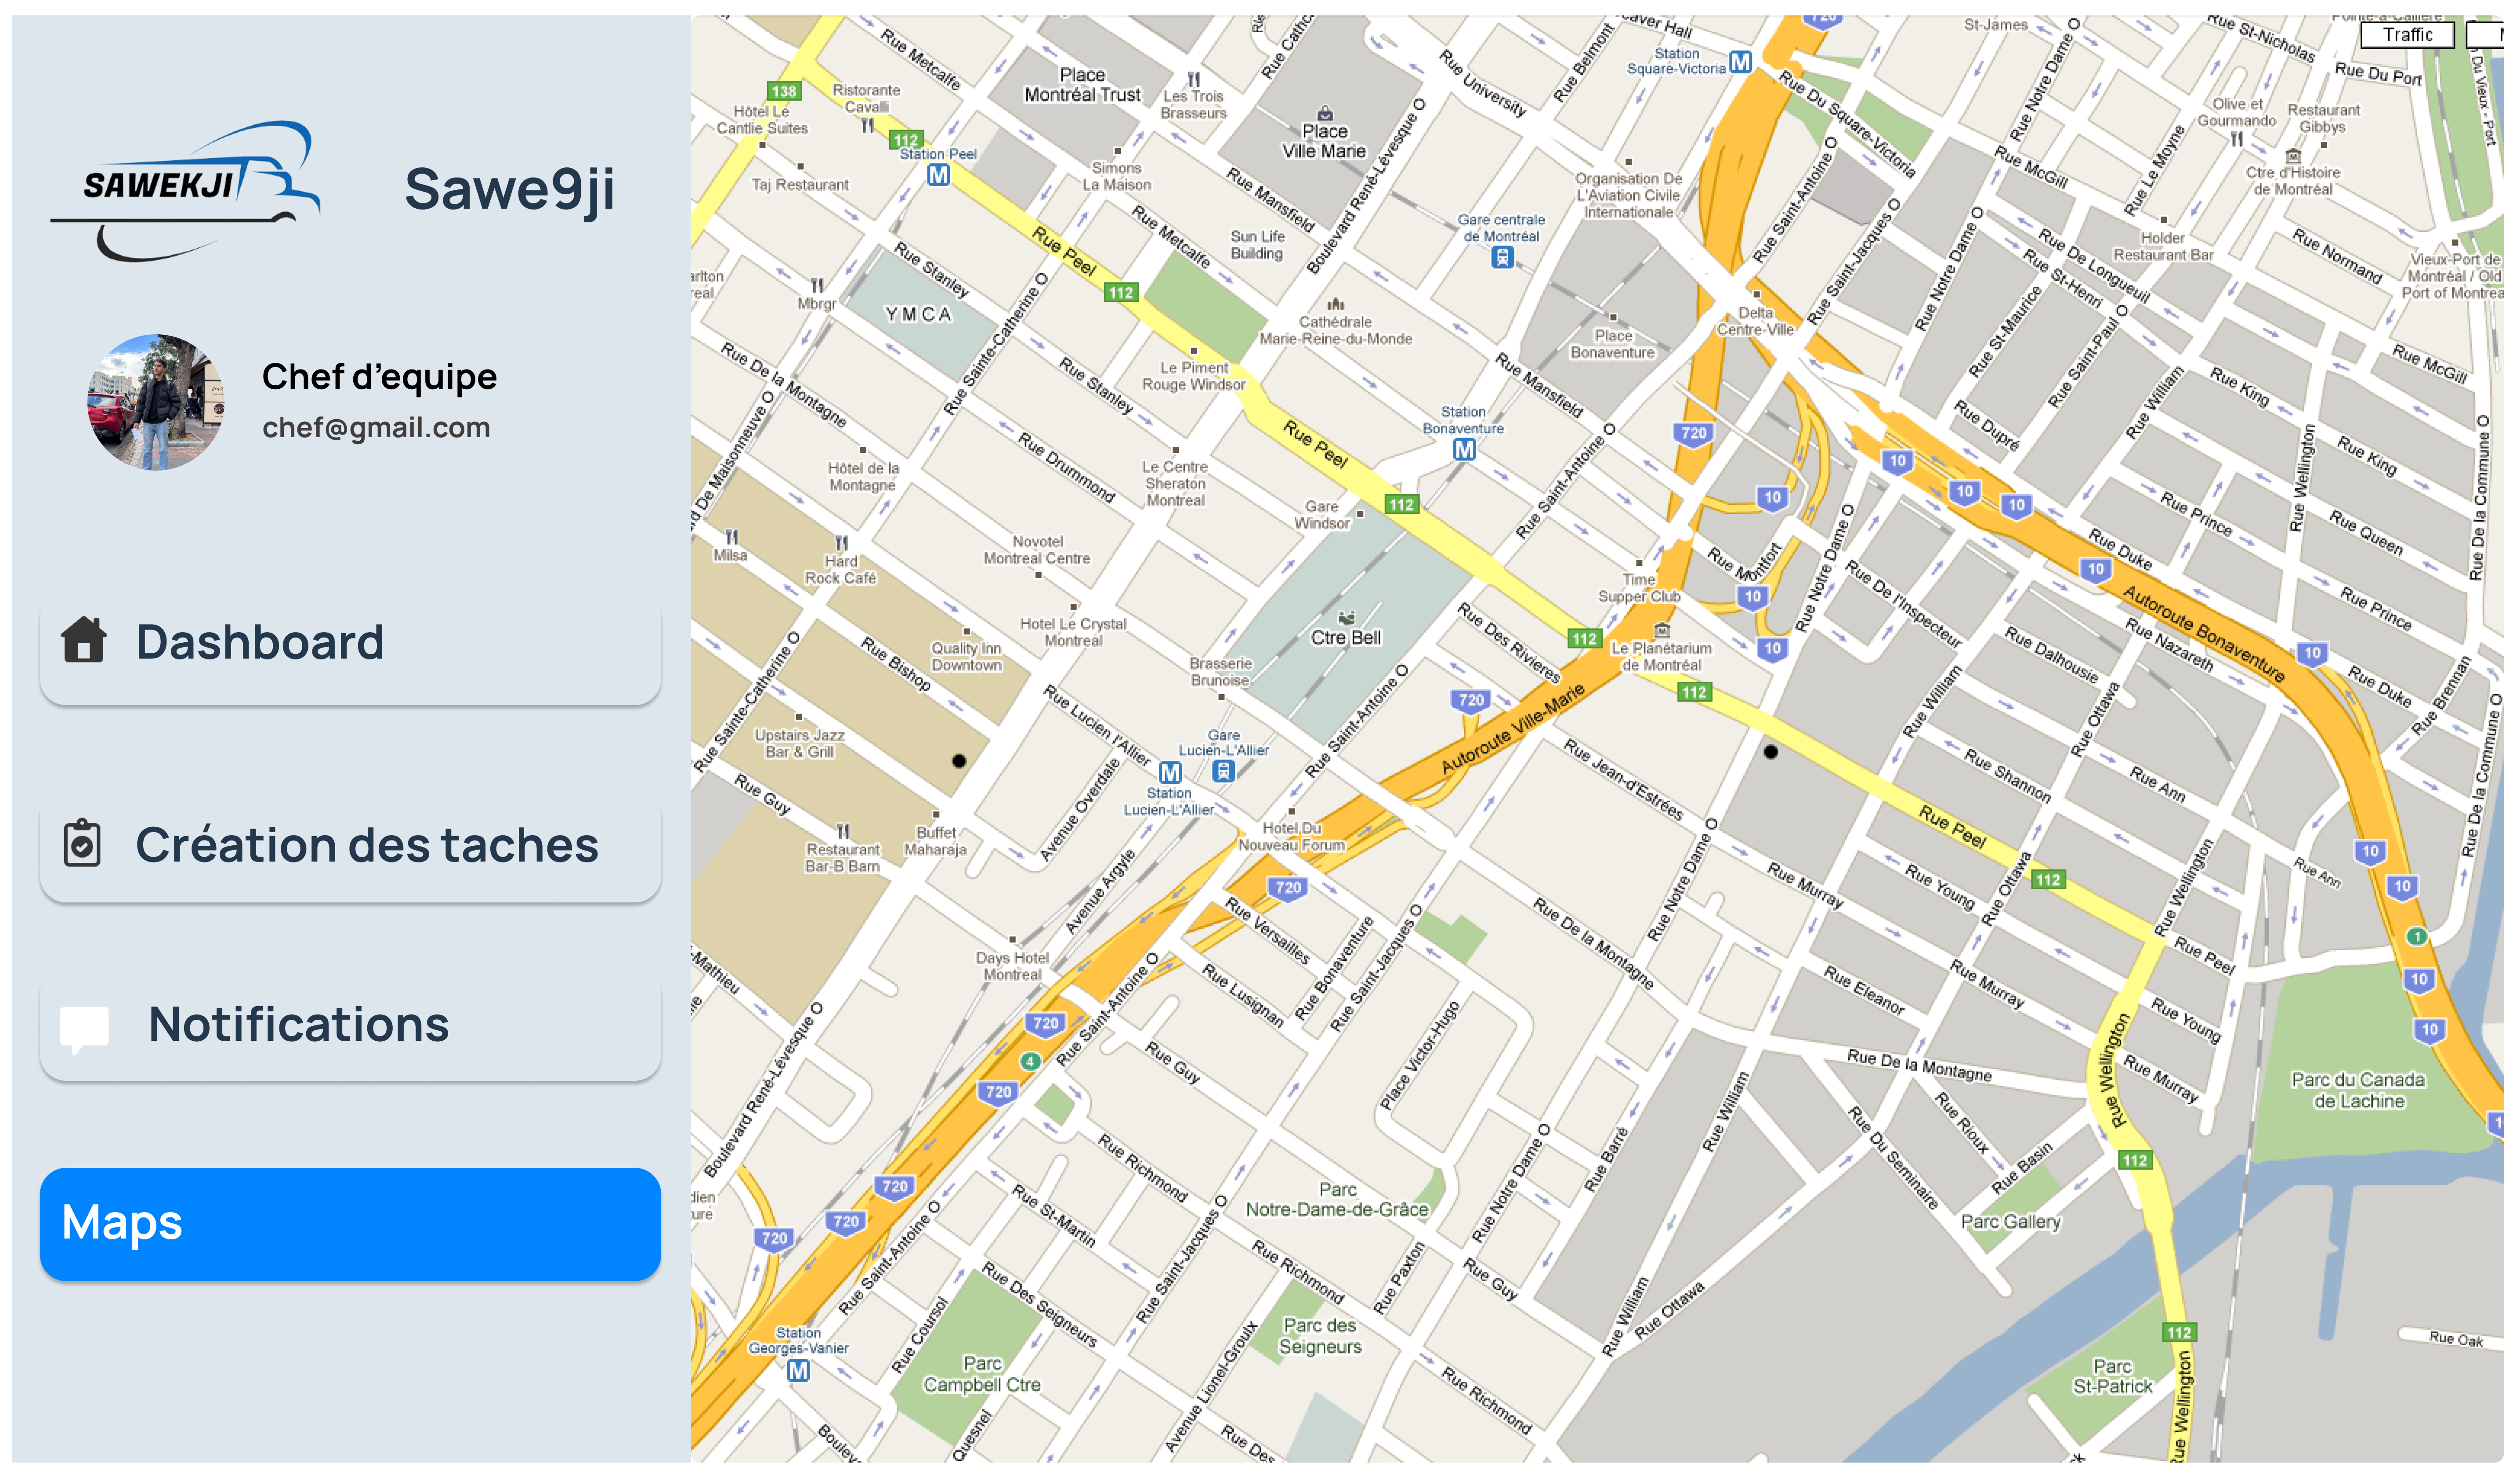
\includegraphics[width=1\textwidth, height=6cm]{chap2.images/maps web.png}
    \caption{map- Web}
  \end{minipage}
  \hfill
  \begin{minipage}[t]{0.38\textwidth}
    \centering
    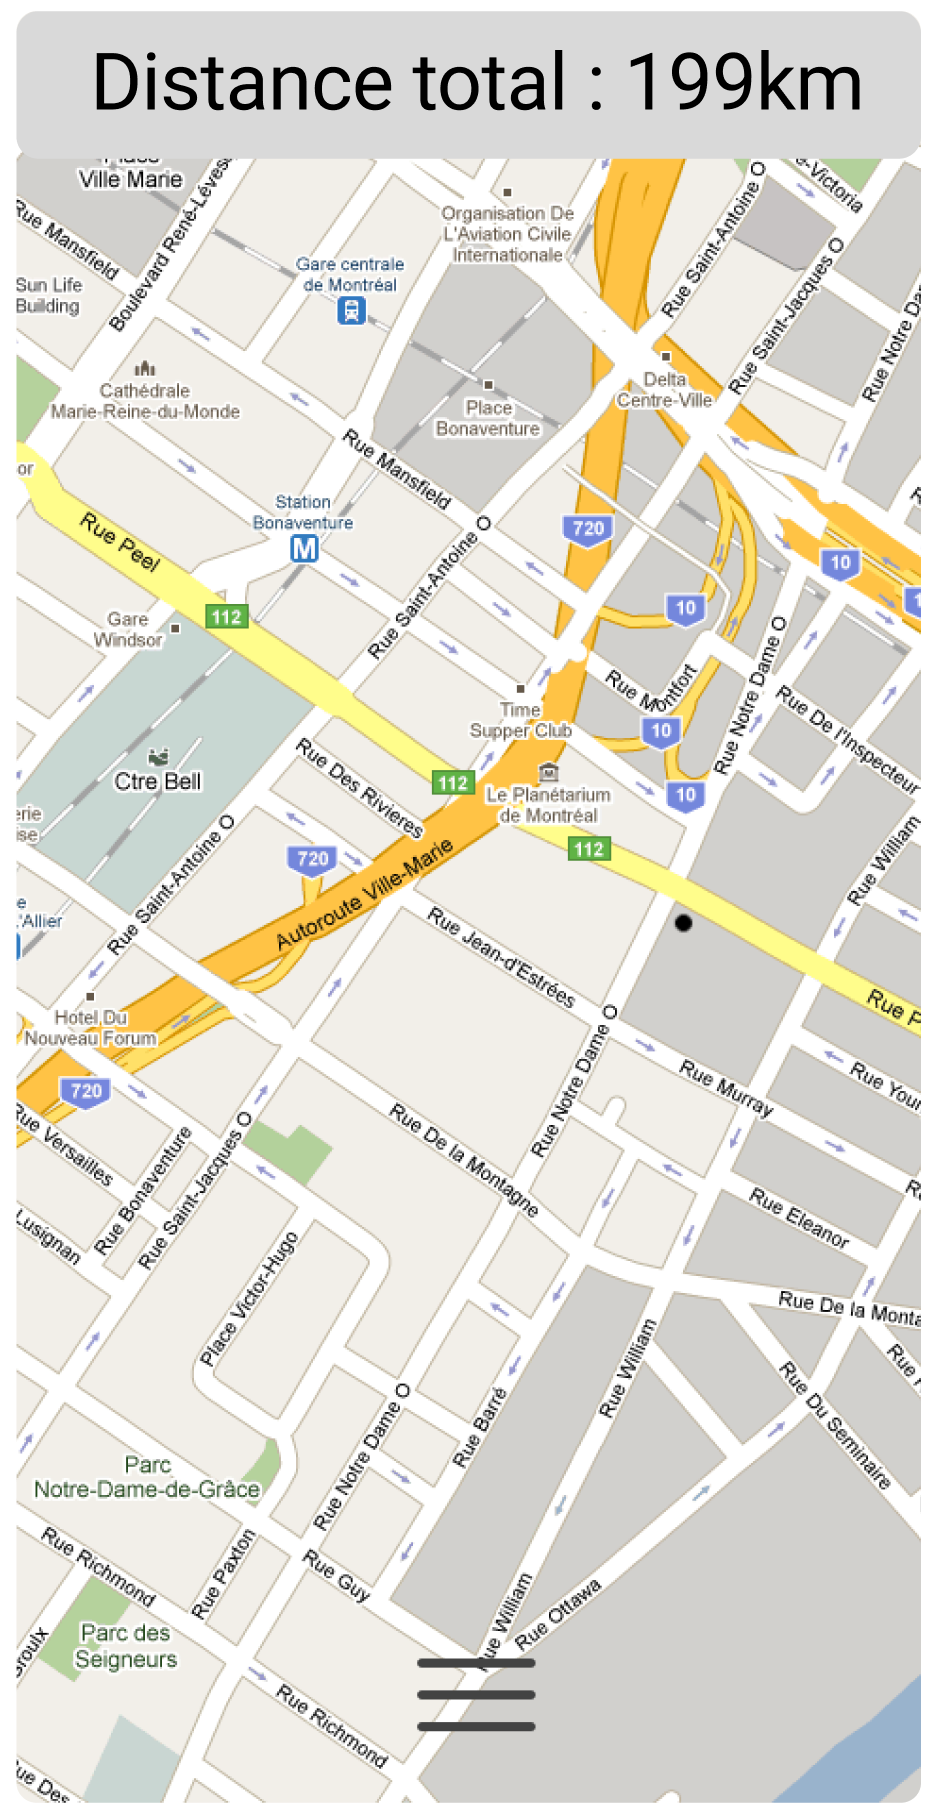
\includegraphics[width=0.6\textwidth, height=6cm]{chap2.images/map mobile.png}
    \caption{\centering{map - Mobile}}
  \end{minipage}
\end{figure}


%__________________________________________________________________________________________________________

\newpage
\subsection{Charte Graphique}

La phase de création de la charte graphique a été précédée par une séance de brainstorming afin de choisir la palette adéquate ainsi que le nom et le logo de l’application.

\begin{figure}[h!]
  \centering
  \begin{minipage}[t]{0.45\textwidth}
    \centering
    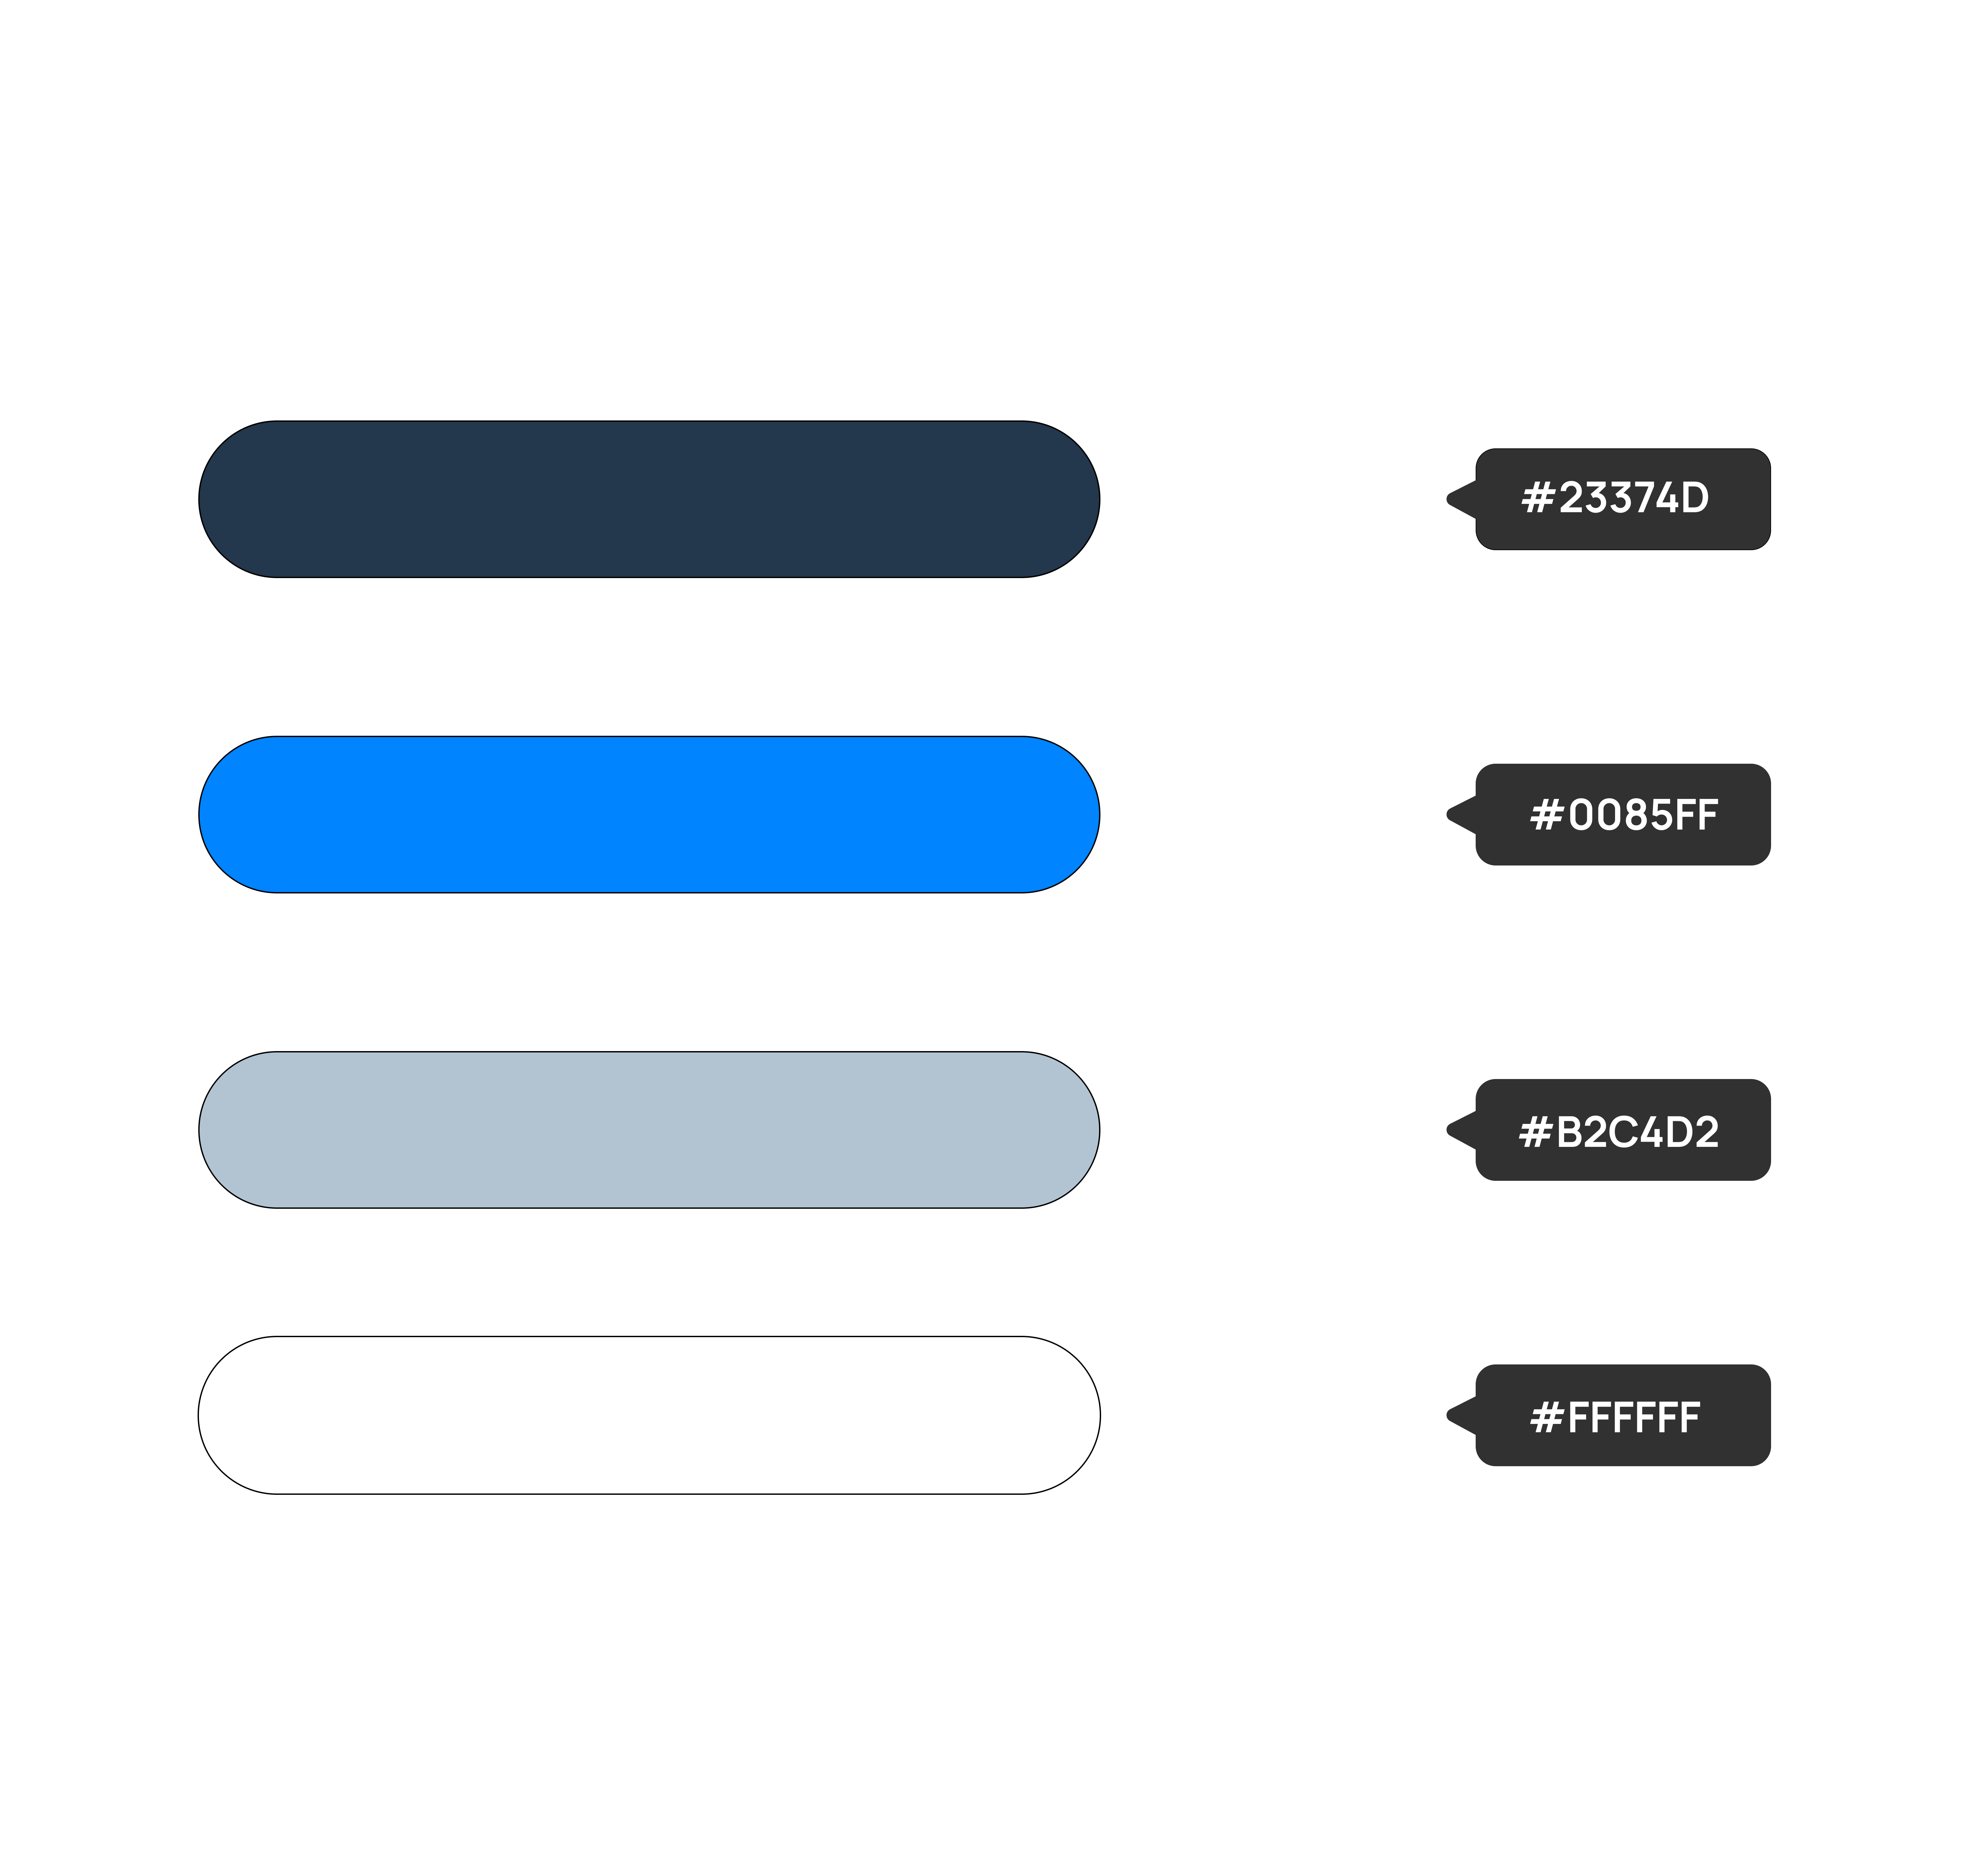
\includegraphics[width=1\textwidth]{chap2.images/palette.png}
    \caption{la palette de couleurs}
  \end{minipage}
  \hfill
  \begin{minipage}[t]{0.45\textwidth}
    \centering
    
\includegraphics[width=0.8\textwidth]{chap2.images/logo.png}
    \caption{\centering{logo}}
  \end{minipage}
\end{figure}
%__________________________________________________________________________________________________________

\subsection{Plan de l'application}
Dans cette section nous exposerons, dans les figures 2.5, 2.6, 2.7 et 2.8 l'organigramme des interfaces de l'application de nos profils d'acteurs à savoir: L'administrateur de l'application, le chauffeur, le mécanicien  et le chef d'equipe .\\

\subsubsection{Diagramme de flux utilisateur}
Le flux utilisateur est une représentation visuelle du chemin qu'un utilisateur suit pour atteindre l’objectif d’application . Voici les éléments d'un flux utilisateur : \\

\begin{itemize}[label=$\bullet$]
  \item \textbf{Flèches d'option de transition}: Ces flèches représentent les différentes options de choix que l'utilisateur peut faire pour avancer ou reculer dans le flux utilisateur.

  \item \textbf{Page}: Cela représente une seule page avec laquelle un utilisateur interagit.

  \item \textbf{Section dans la page}: Il s'agit de zones spécifiques sur une page, telles qu'un formulaire ou un menu de navigation.

  \item \textbf{Point final}: C'est le résultat final du flux utilisateur.

  \item \textbf{Entrée d'informations}: Ce sont les entrées requises de l'utilisateur, telles que remplir un formulaire ou saisir des informations de connexion.

  \item \textbf{Décision}: Ils représentent un choix ou une décision que l'utilisateur doit prendre.

  \item \textbf{Traitement des données}: Cela représente tout traitement de données qui se produit pendant le flux utilisateur.
\end{itemize}

\bigskip
\textbf{Flux utilisateur ( Définition des éléments ):}
\begin{figure}[htbp]
  \centering
  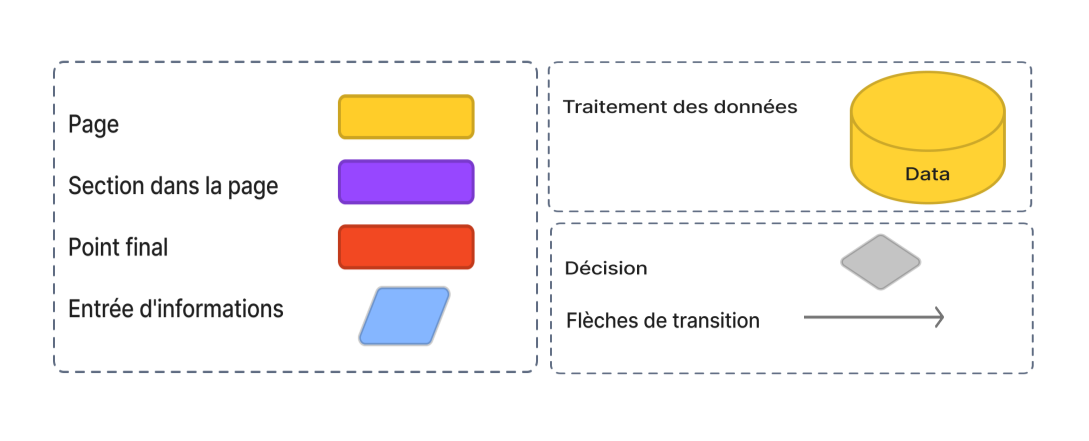
\includegraphics[width=0.9\textwidth]{chap2.images/user flow ( Définition des éléments ).png}
  \caption{Flux utilisateur : Définition des éléments}
\end{figure}


\bigskip
\textbf{Vue globale sur les flux d’utilisateurs :}
\begin{figure}[htbp]
  \centering
  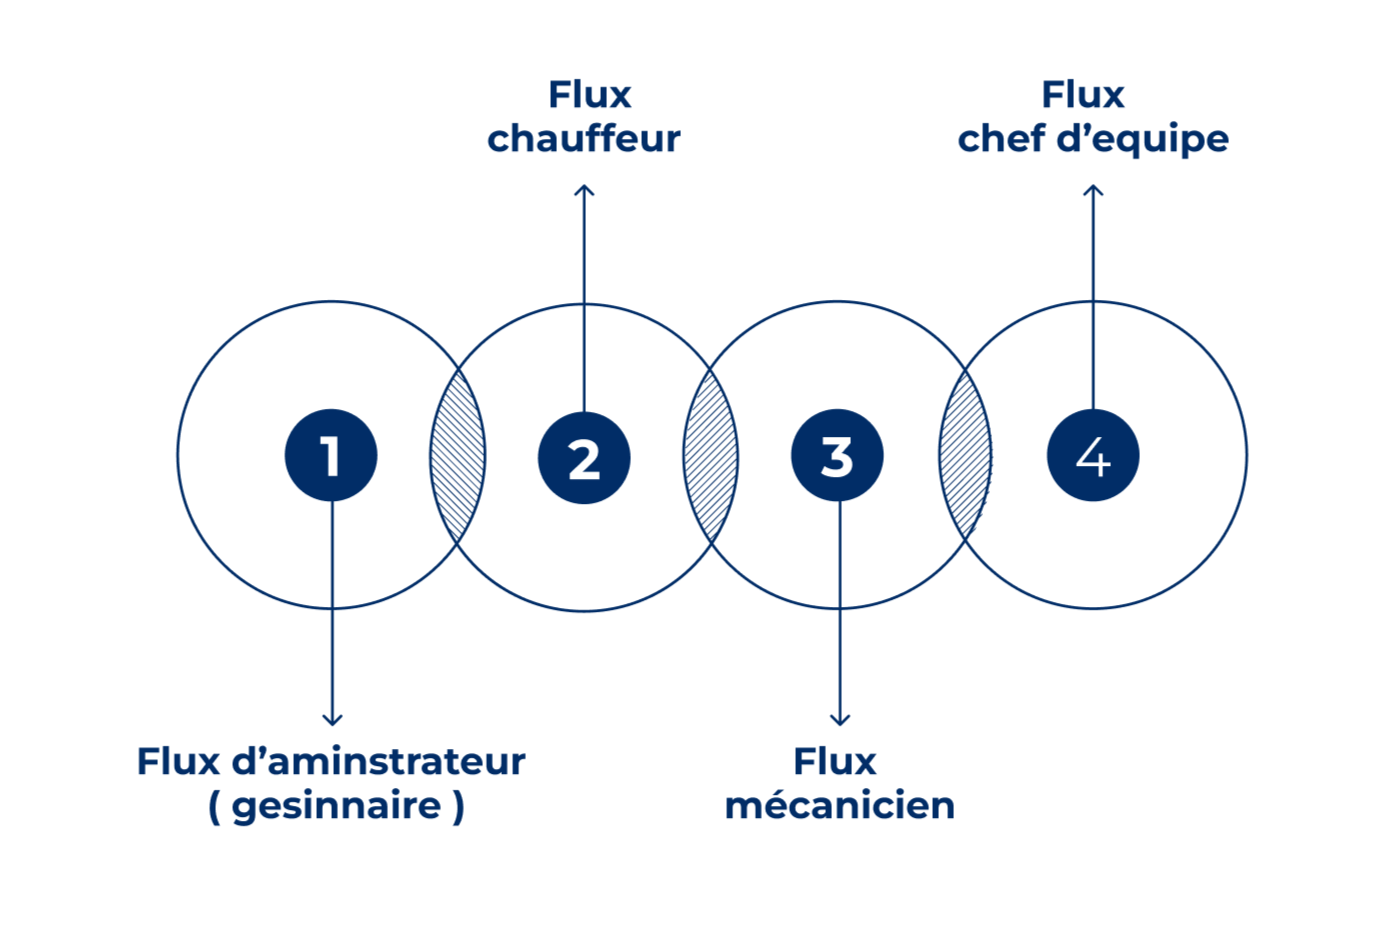
\includegraphics[width=0.7\textwidth]{chap2.images/vue global user flow.png}
  \caption{Vue globale sur les flux d'utilisateurs}
\end{figure}




\newpage
\subsubsection{Flux administrateur}
\begin{figure}[htbp]
  \centering
  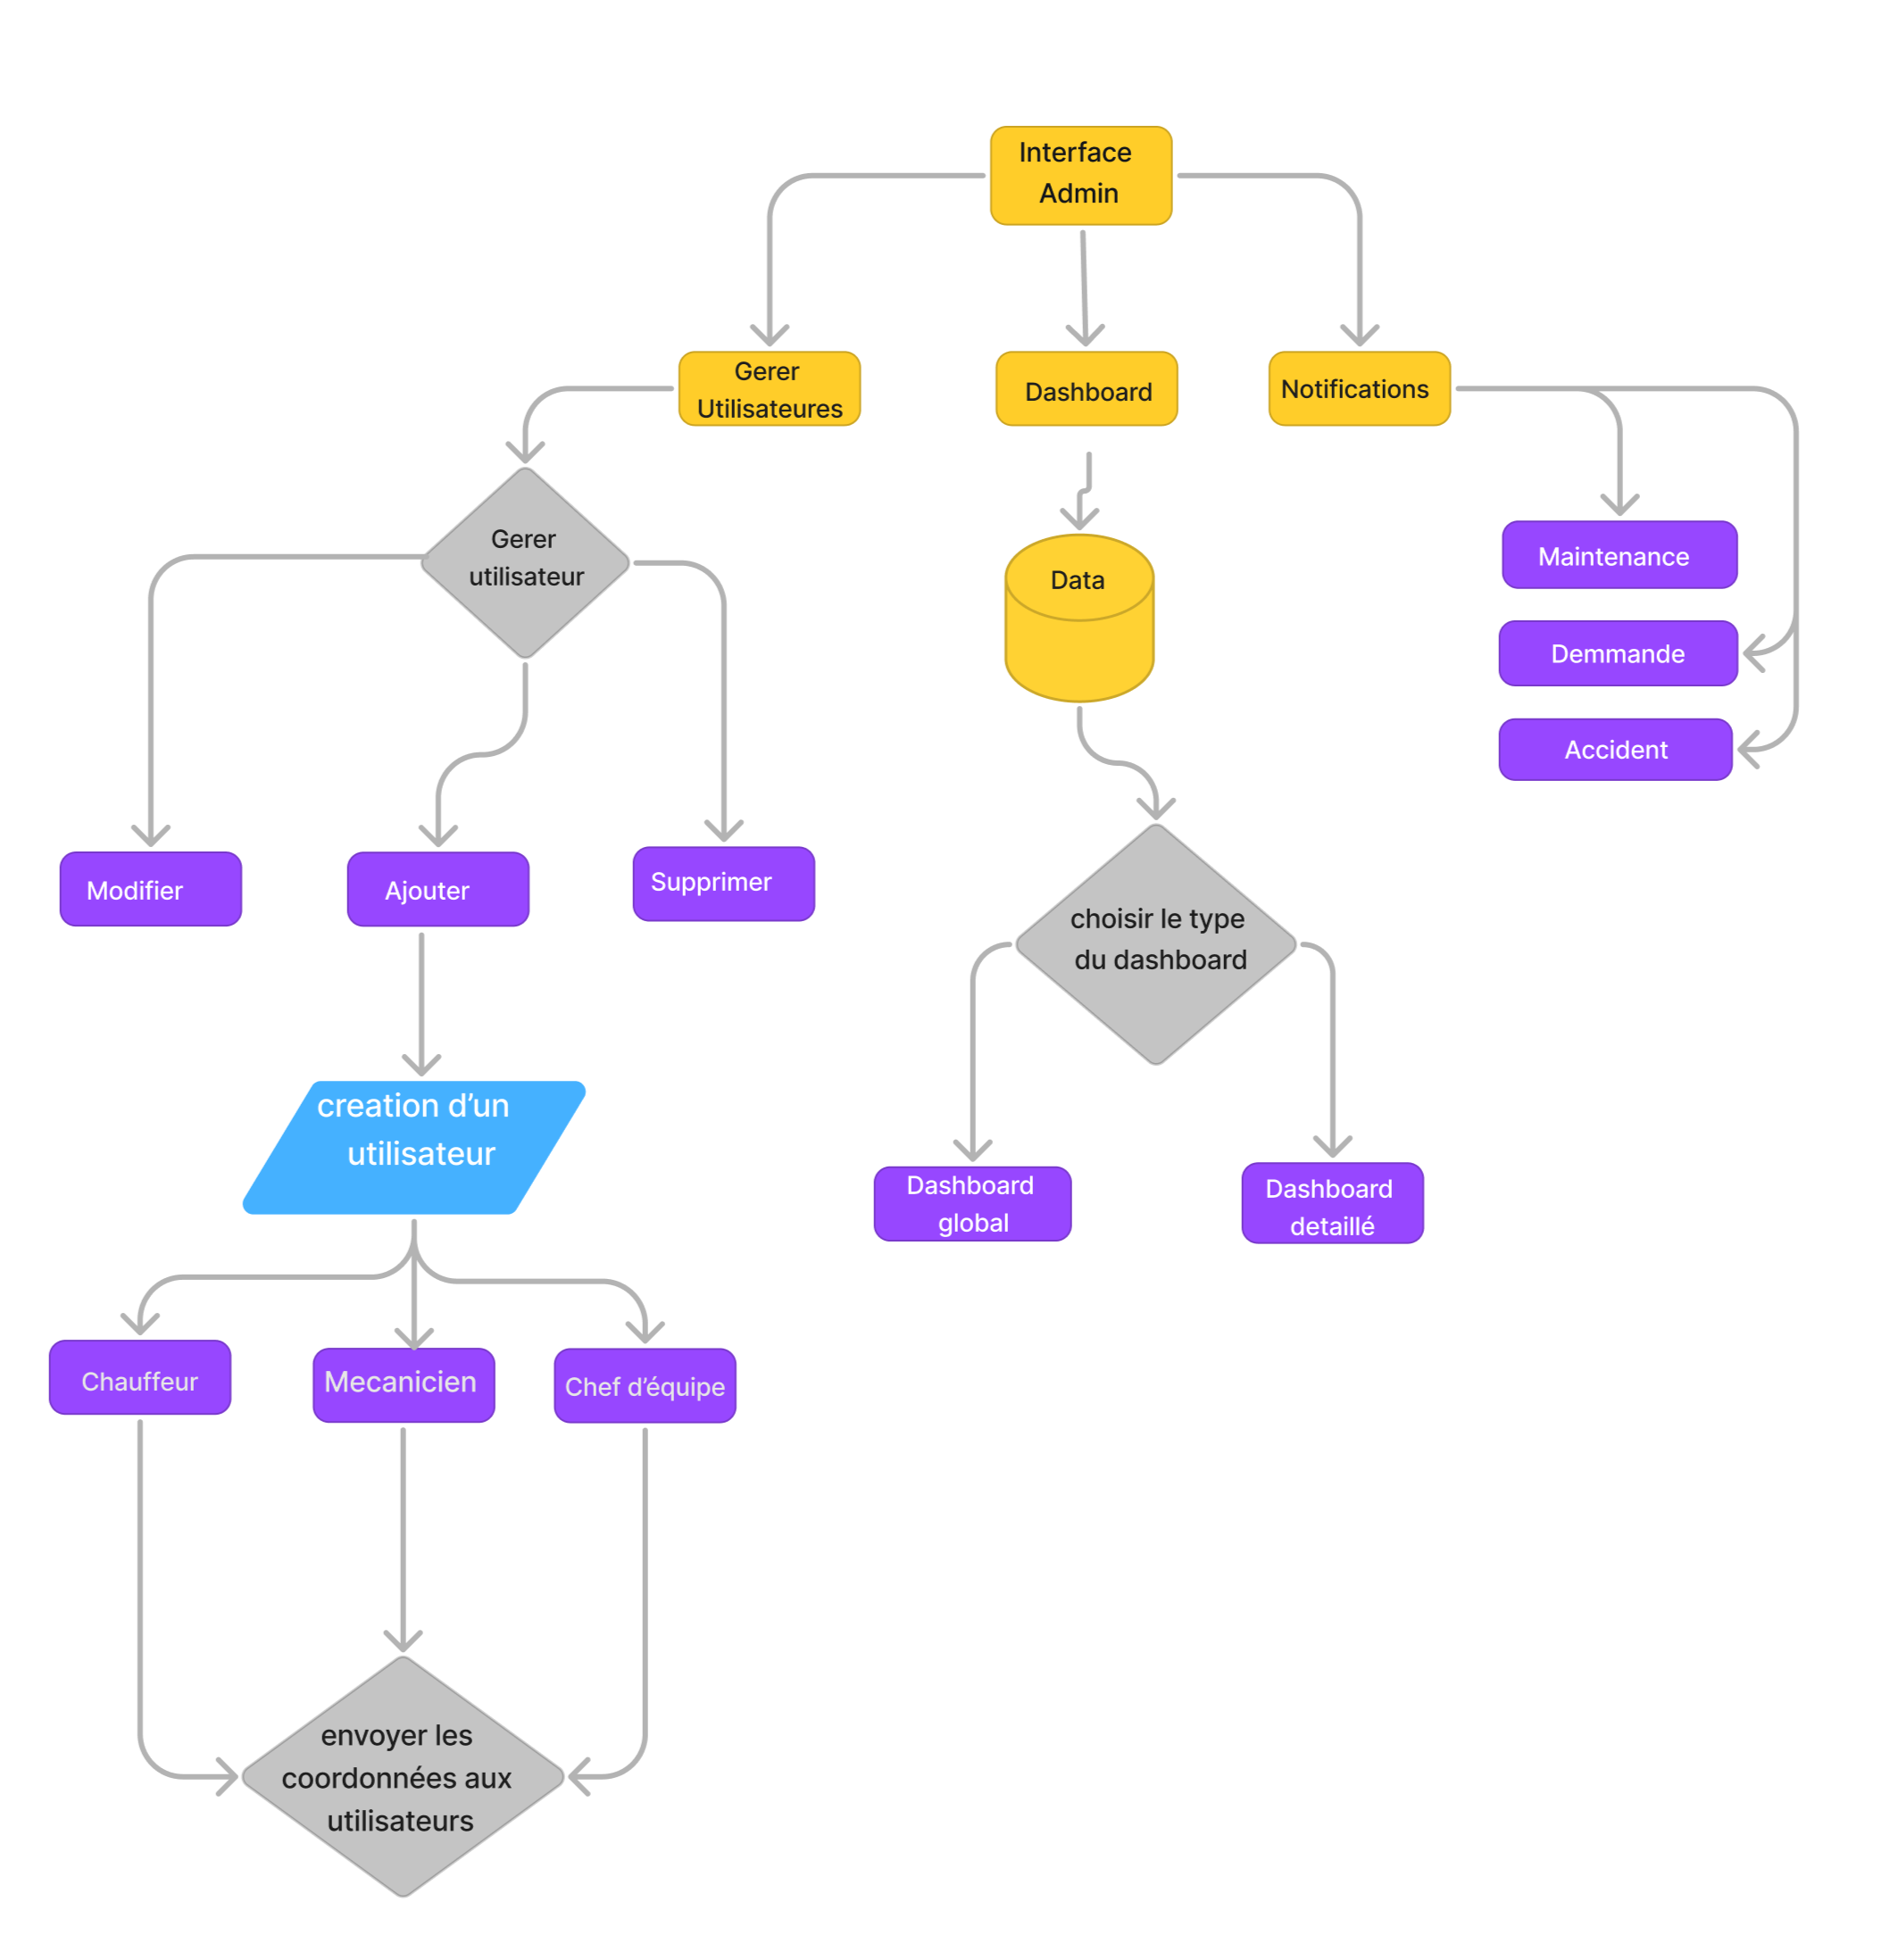
\includegraphics[width=1\textwidth,height=17cm]{chap2.images/org admin.png}
  \caption{Organigramme des interfaces du l'administrateur }
\end{figure}


\newpage
\subsubsection{Flux chauffeur}
\begin{figure}[htbp]
  \centering
  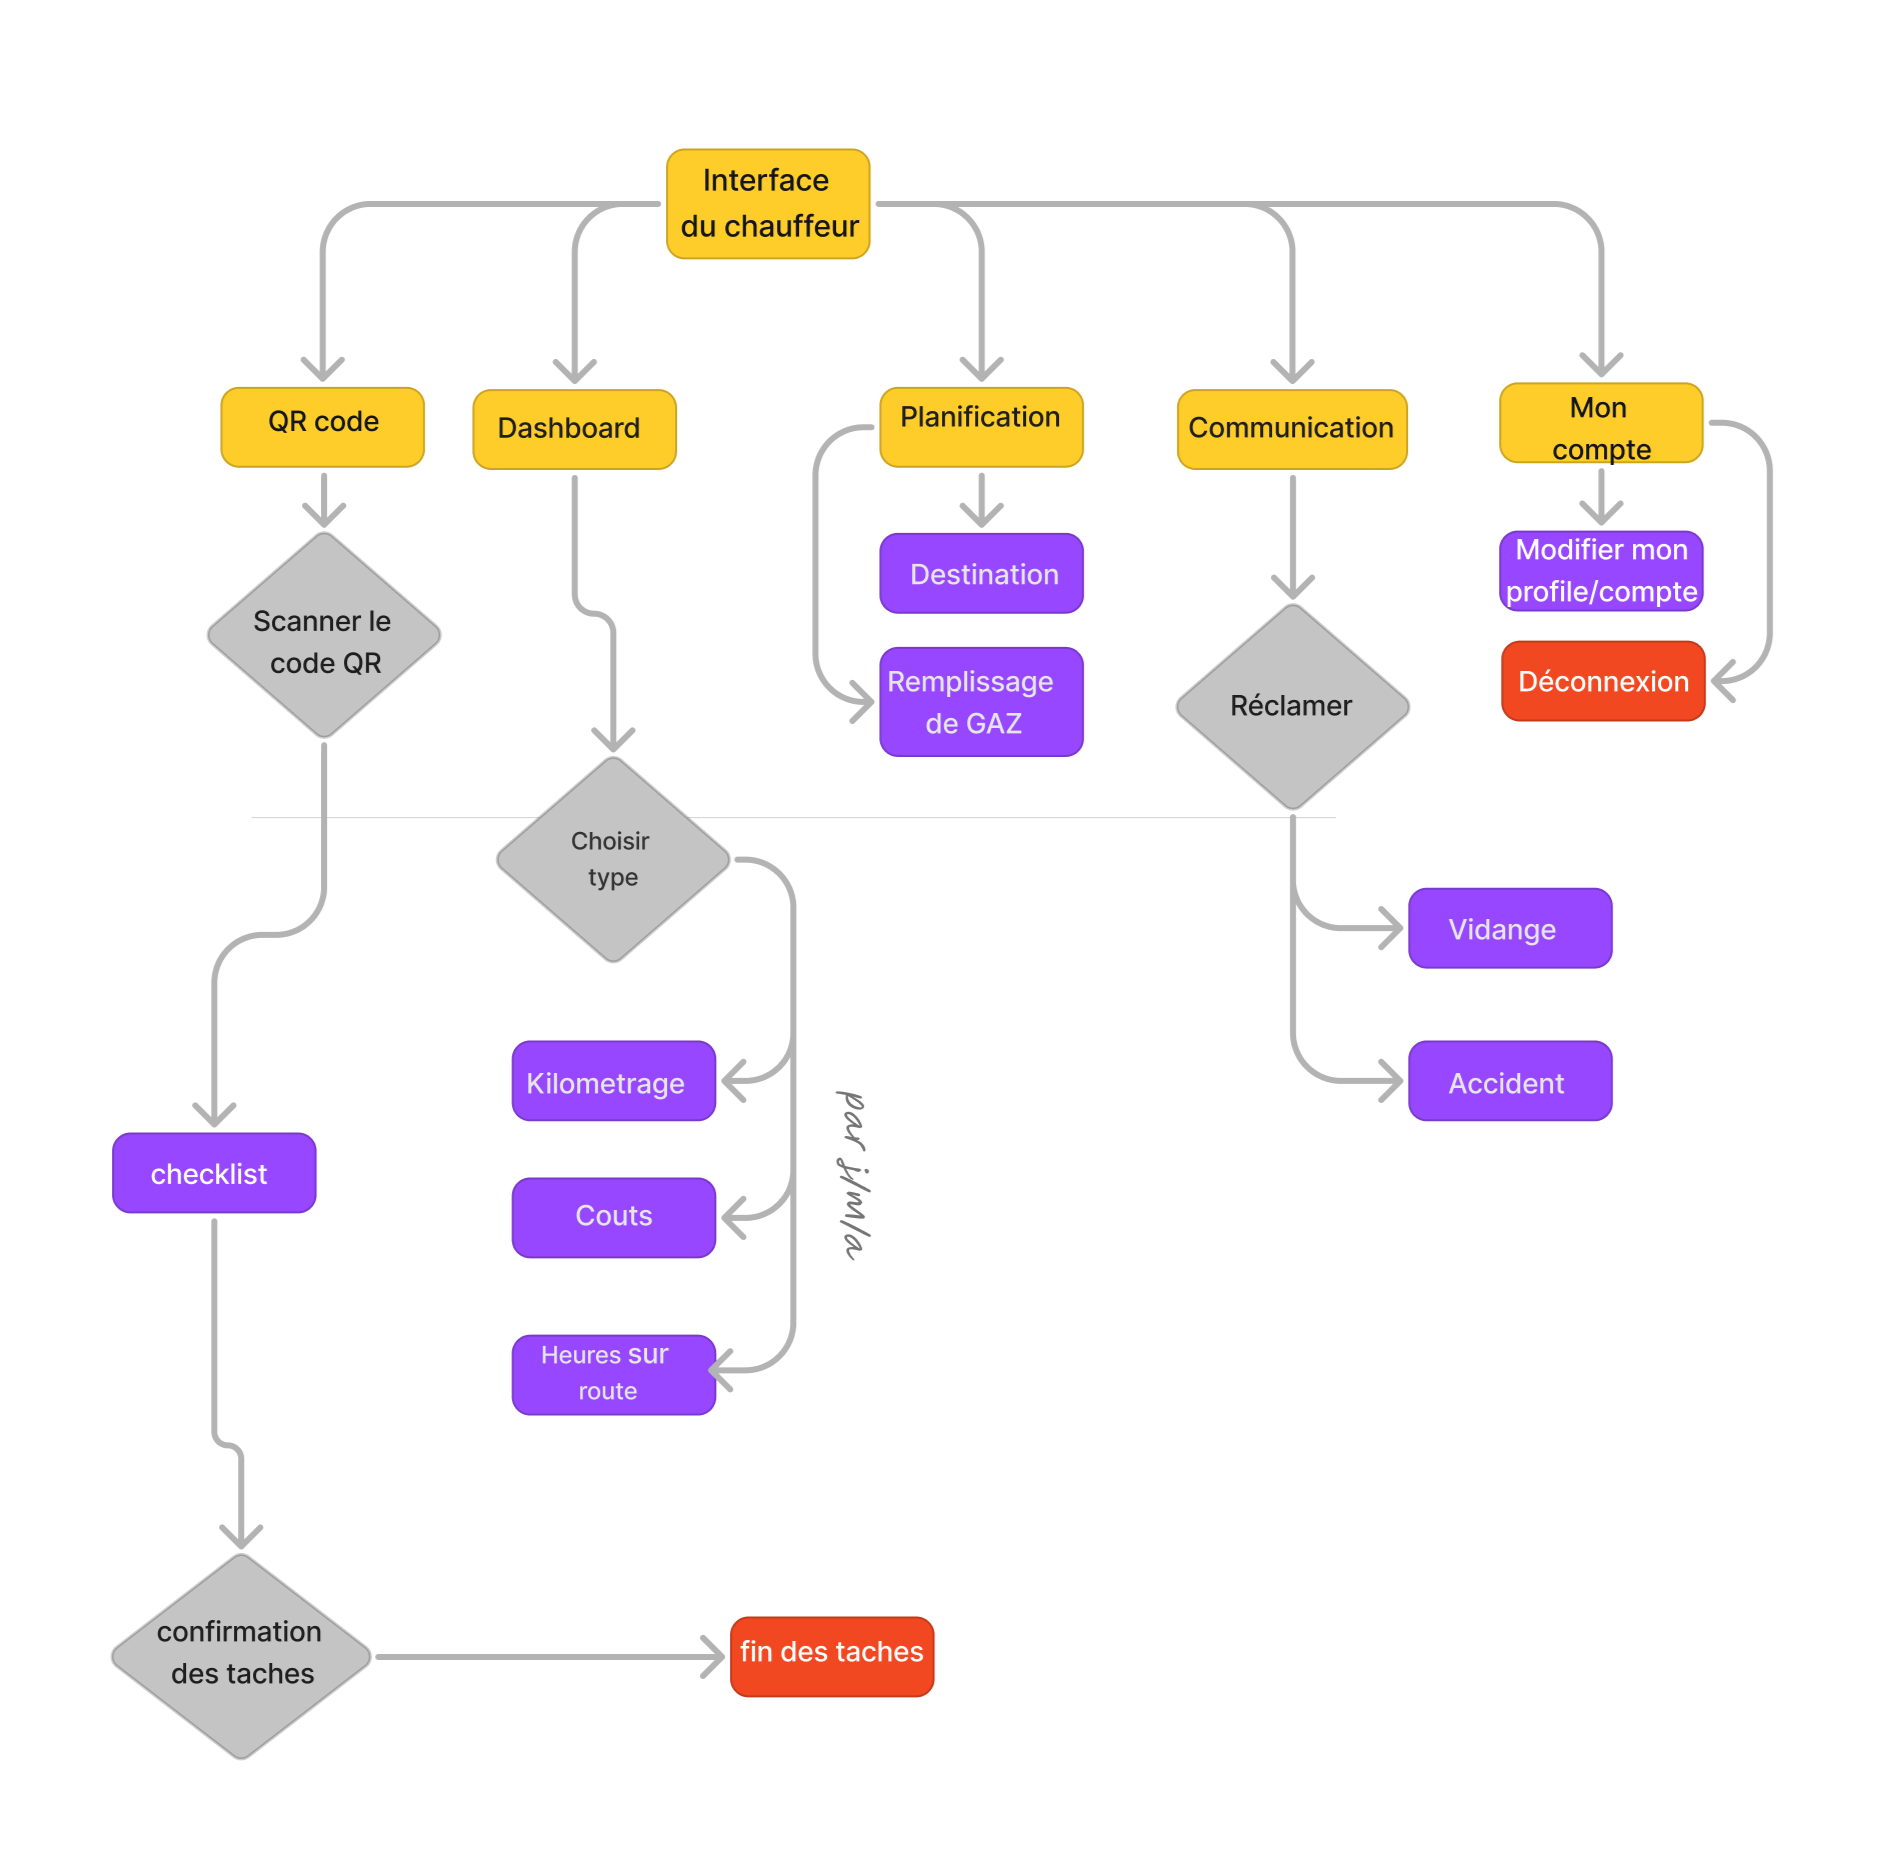
\includegraphics[width=1\textwidth,height=17cm]{chap2.images/org chauffeur.png}
  \caption{Organigramme des interfaces du chauffeur}
\end{figure}

\newpage
\subsubsection{Flux mécanicien}
\begin{figure}[htbp]
  \centering
  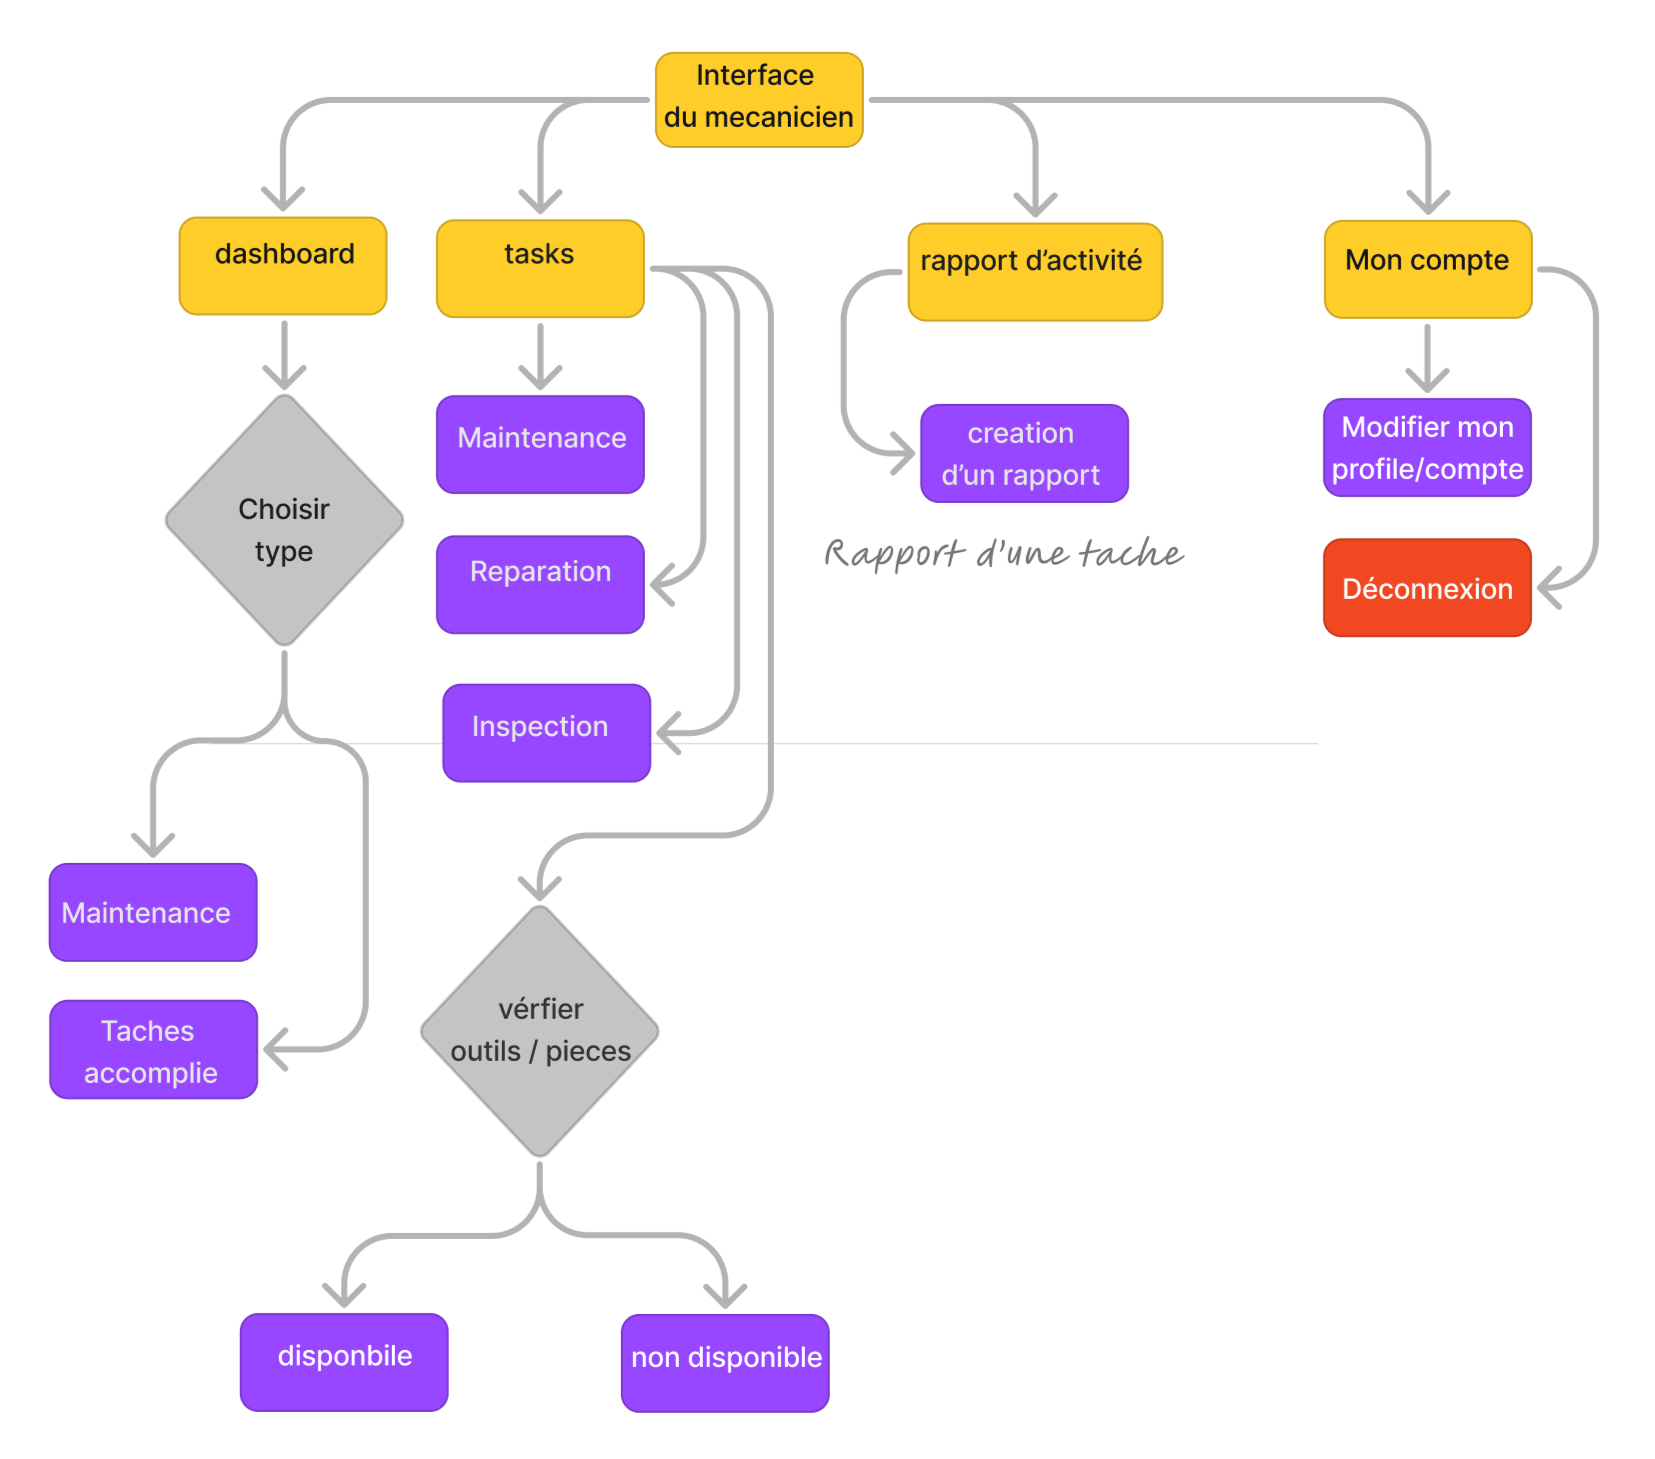
\includegraphics[width=1\textwidth,height=17cm]{chap2.images/org mecanicien.png}
  \caption{Organigramme des interfaces  du mécanicien}
\end{figure}

\newpage
\subsubsection{Flux chef d'équipe}
\begin{figure}[htbp]
  \centering
  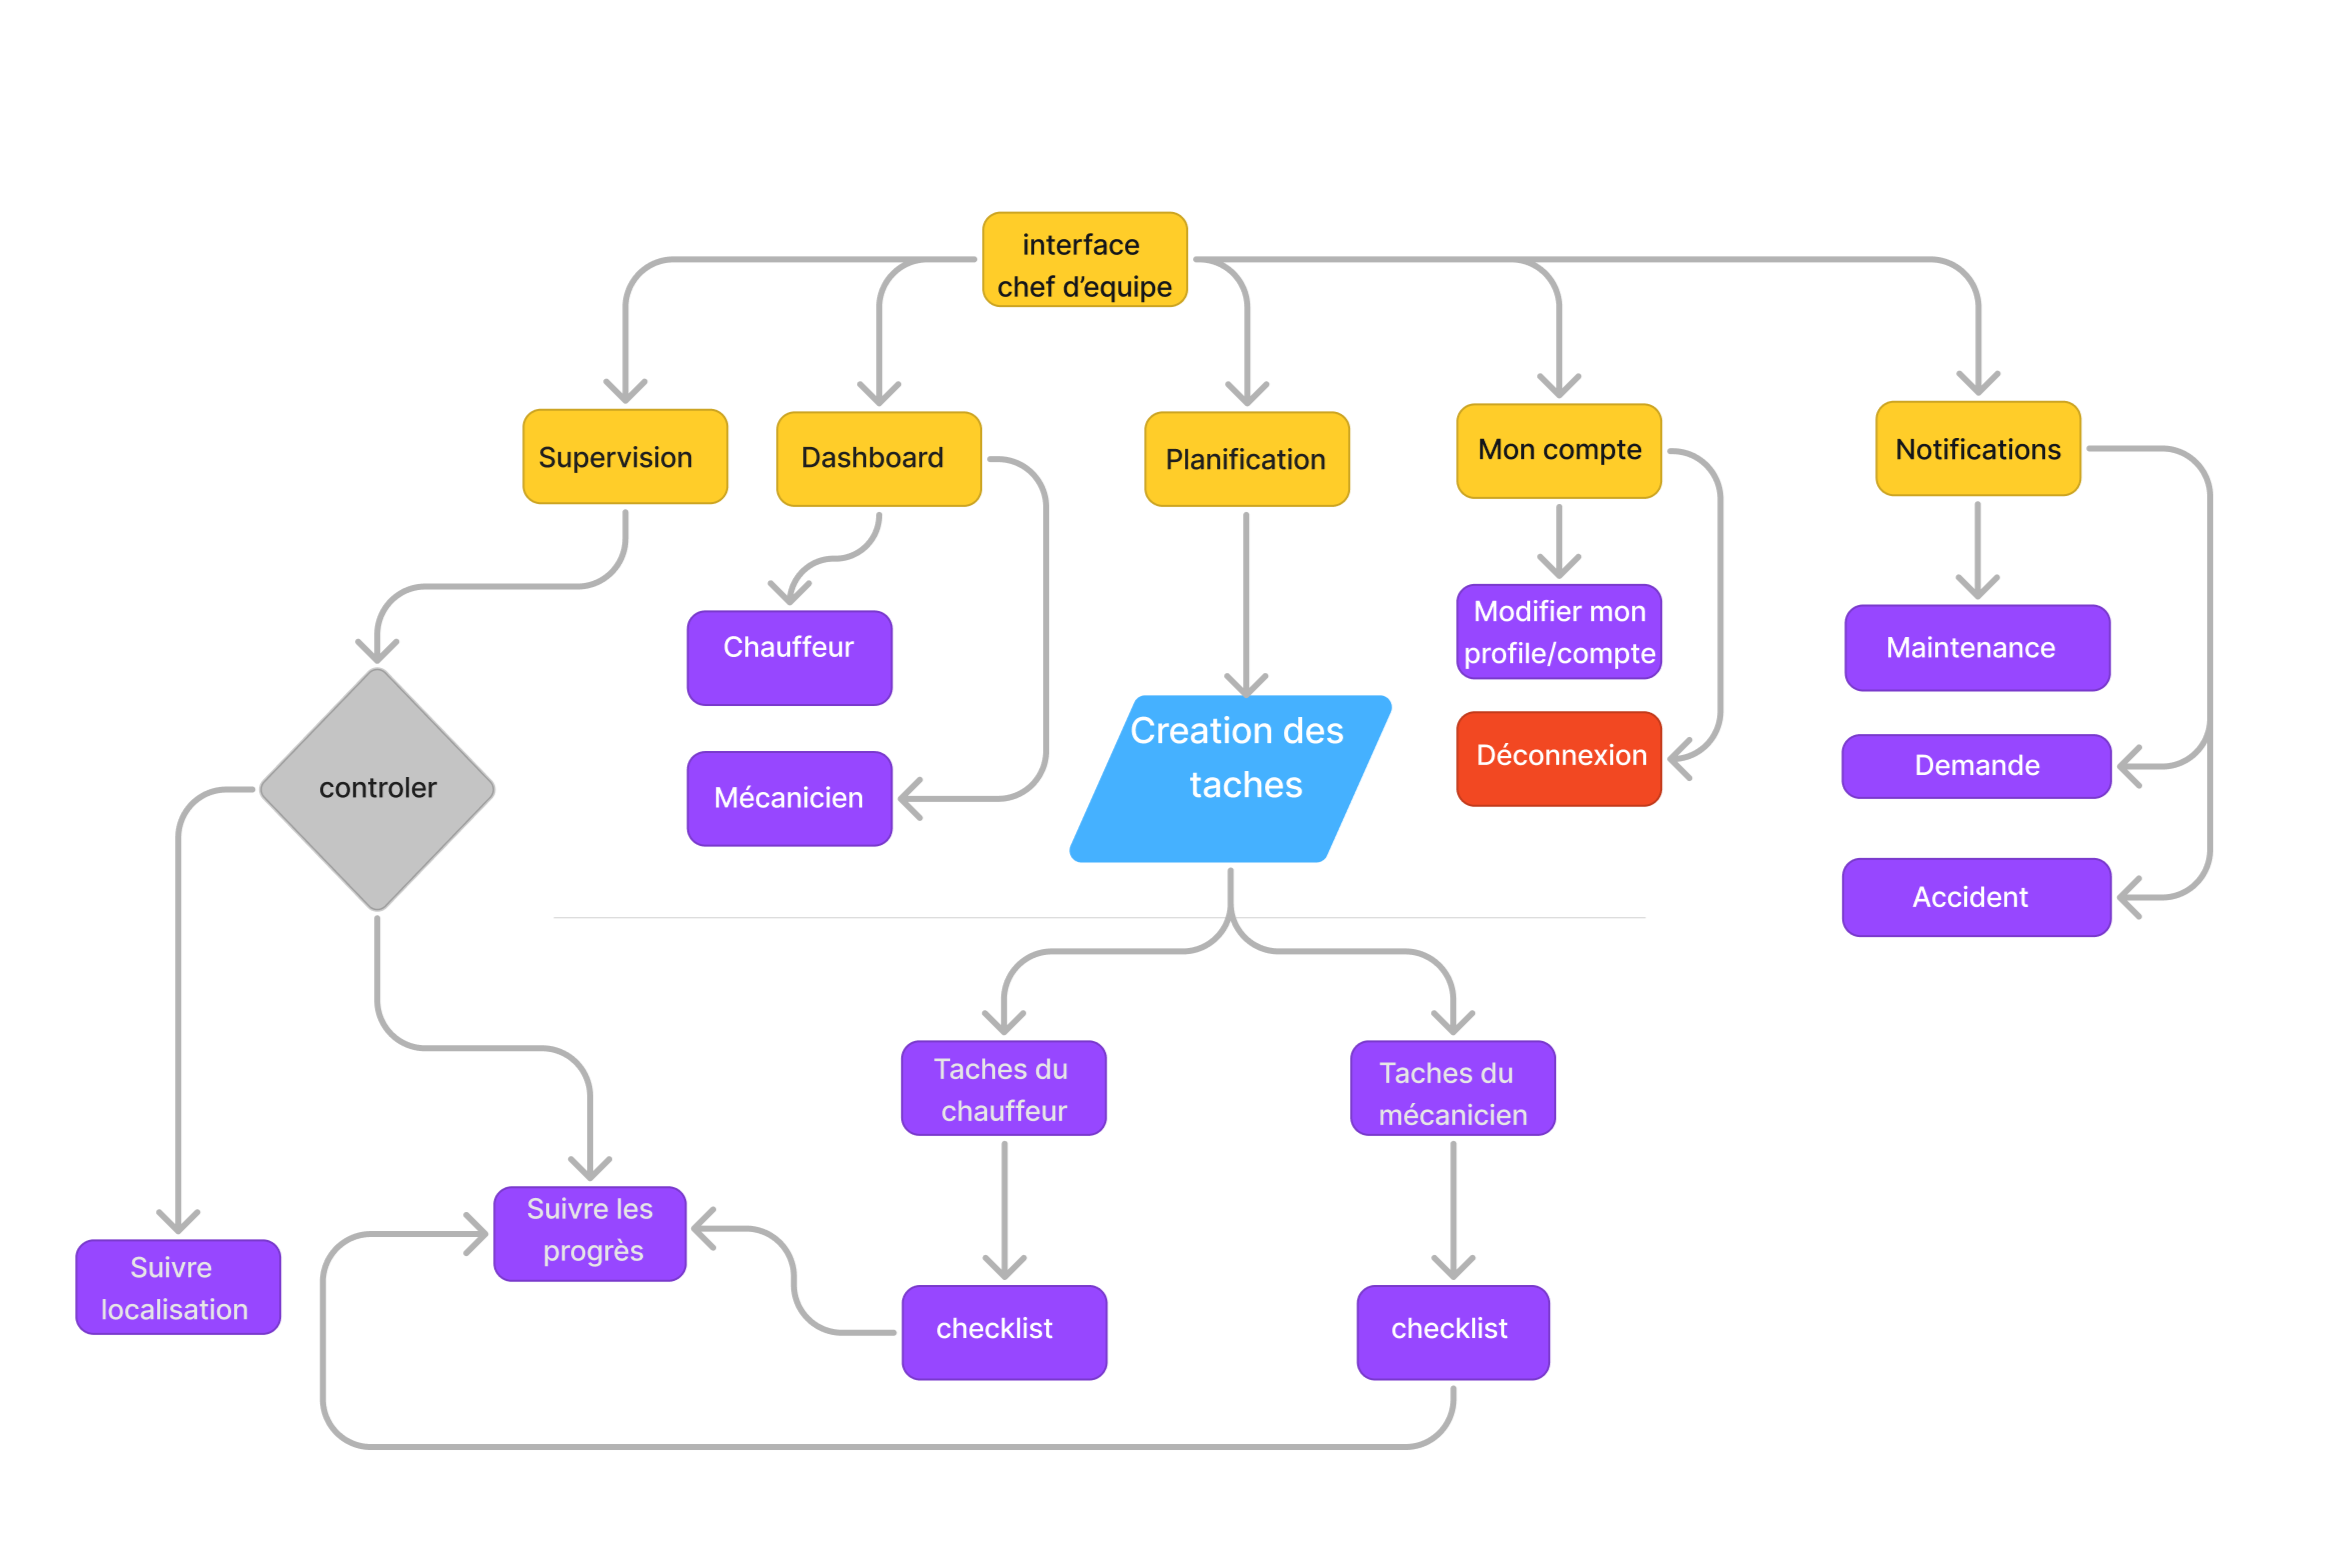
\includegraphics[width=1\textwidth,height=17cm]{chap2.images/org chef d'equipe.png}
  \caption{Organigramme des interfaces du chef d'équipe}
\end{figure}



%_________________________________________________________________________________________________________

\newpage
\subsection{Diagramme de classe du domaine}

La figure 2.21 montre le diagramme de classes du domaine de notre application.








%_________________________________________________________________________________________________________


\newpage
\subsection{Diagramme de Gantt }

Par cette figure 2.20 nous présentons une planification previsionnelle du projet .

\begin{figure}[ht!]
  \centering
  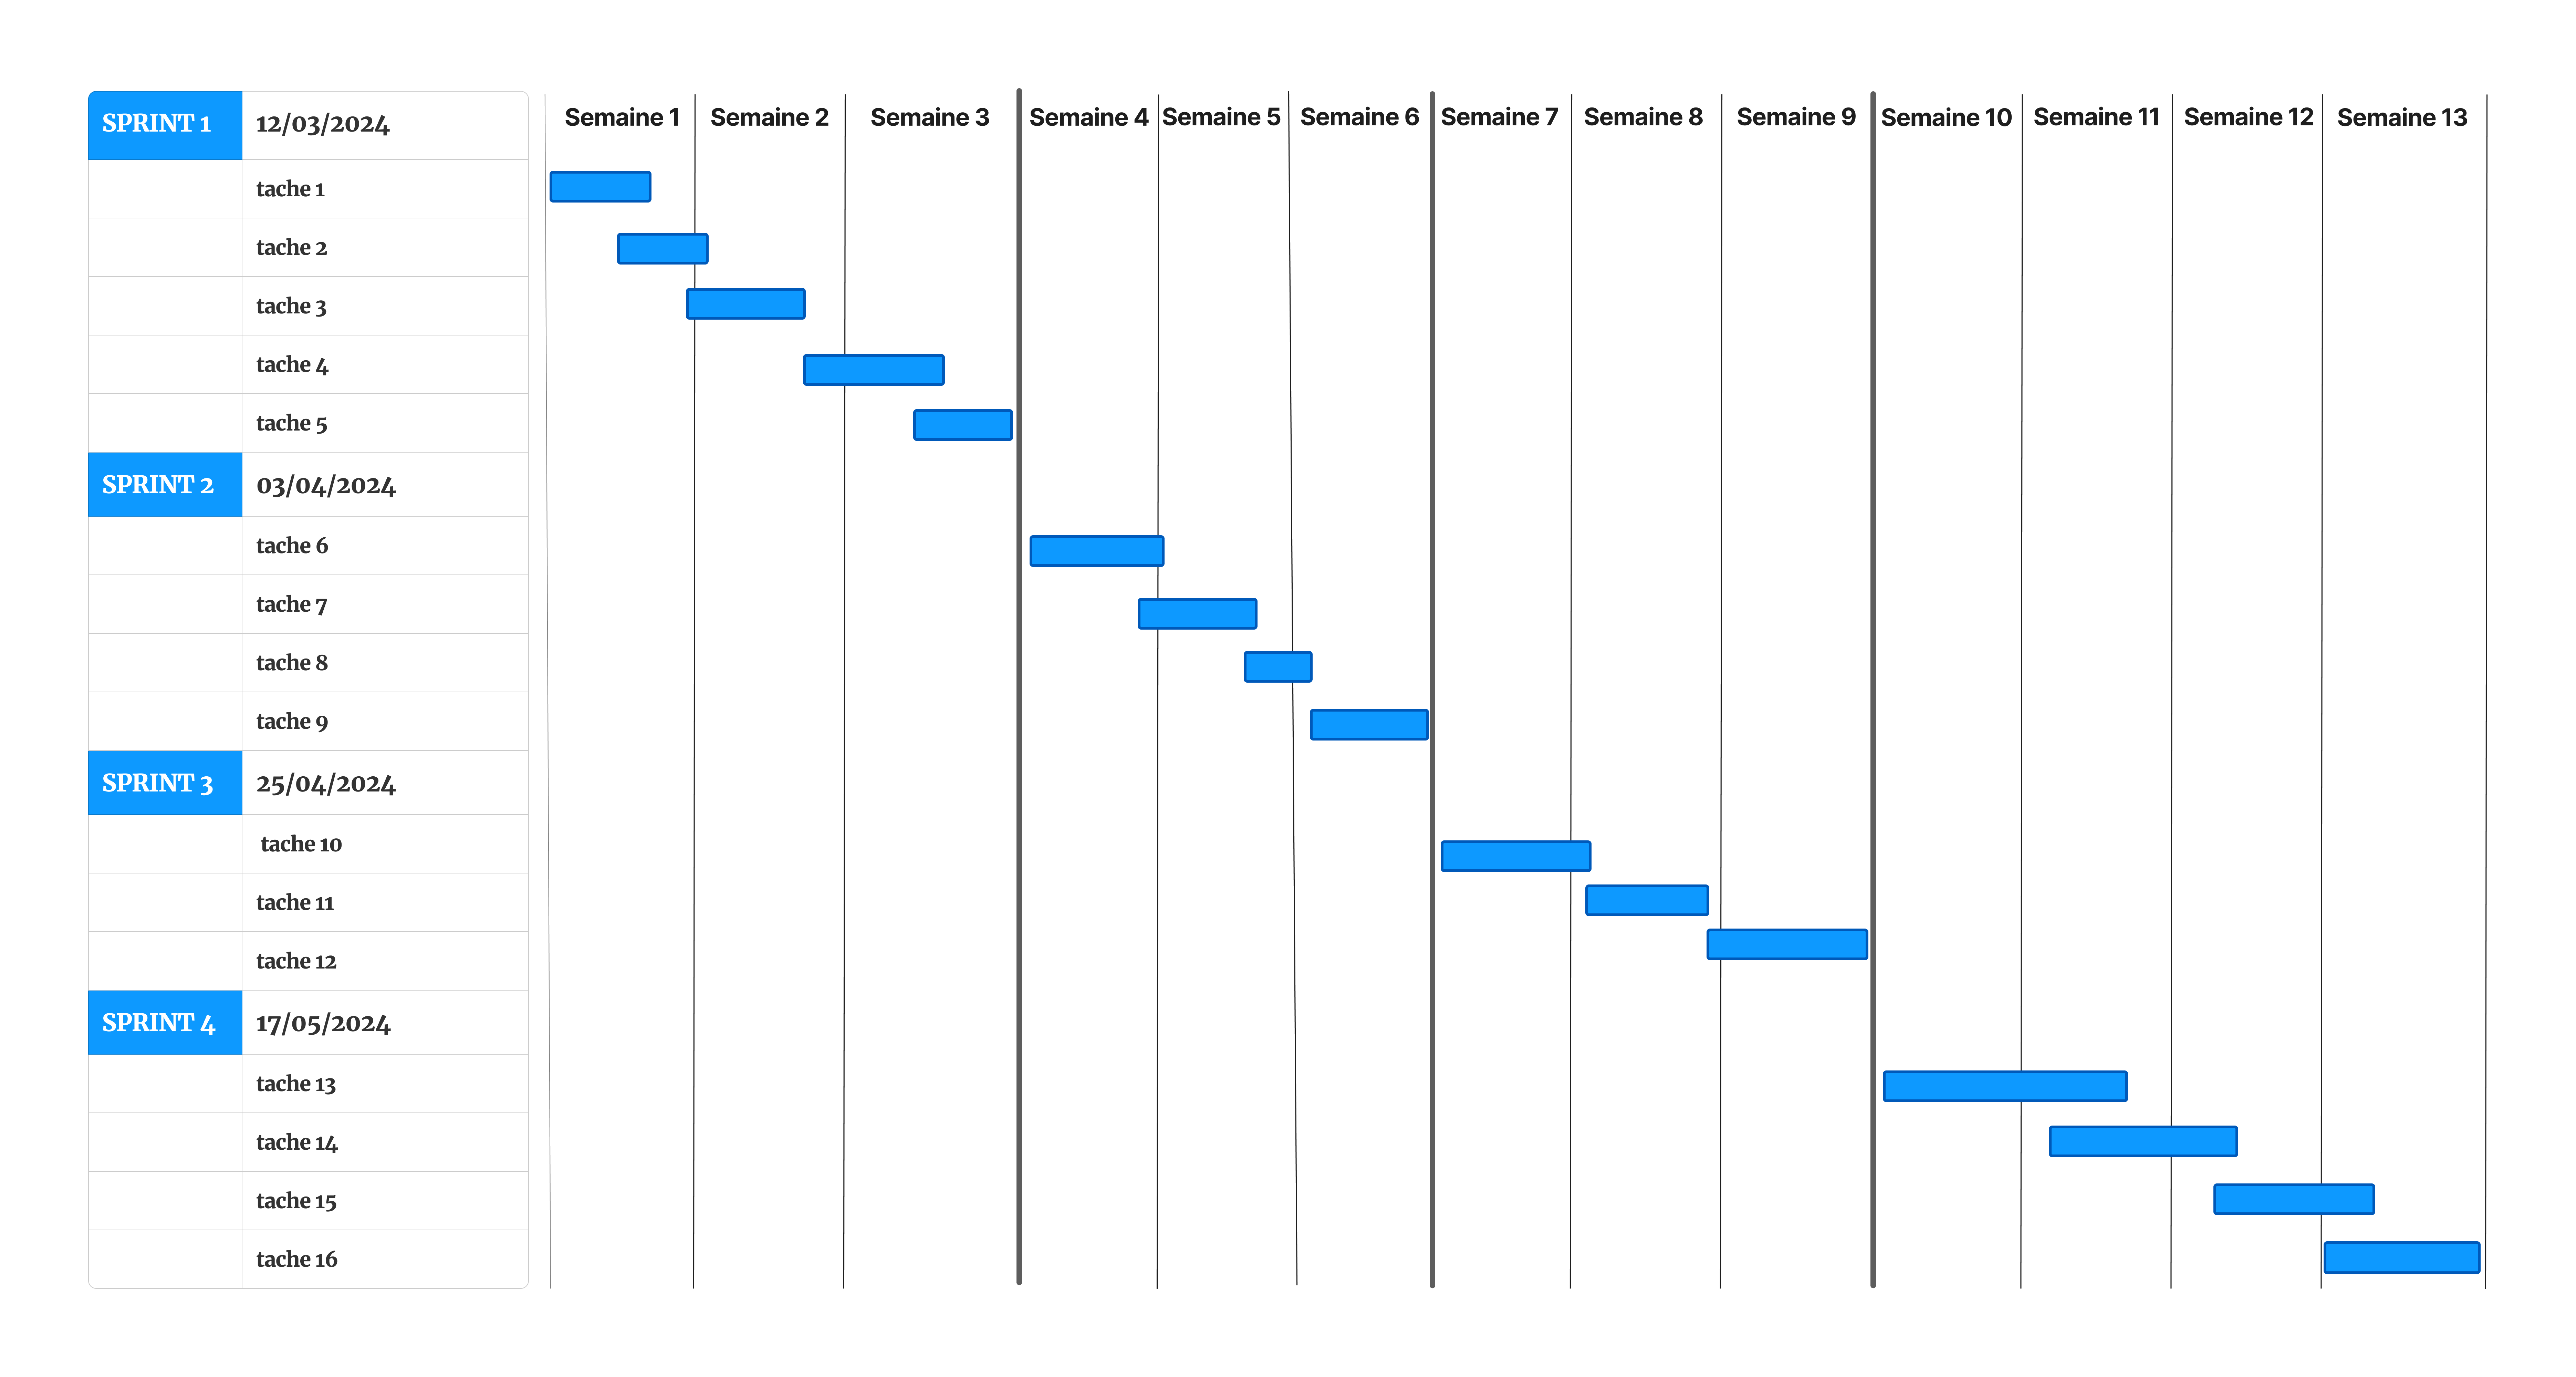
\includegraphics[width=1\textwidth,height=11cm]{chap2.images/diagramme de gantt.png}
  \caption{Diagramme de Gantt}
\end{figure}






%_________________________________________________________________________________________________

\section*{Conclusion}
\addcontentsline{toc}{section}{Conclusion}
\bigskip
\begin{sloppypar}
  Durant ce chapitre, en plus de l'identification  des acteurs, des besoins fonctionnels et non fonctionnels de notre application,  nous avons exposé le premier artéfact de la méthodologie Scrum à savoir le Backlog du produit qui comporte la liste des exigences fonctionnelles et techniques de notre application. Nous avons également identifié les différents rôles au sein de l'équipe du projet et en fin nous avons  exploré le flux utilisateurs de notre application, mettant en évidence les différentes interactions entre les utilisateurs et les fonctionnalités clés de l'application.
  Dans le chapitre suivant, nous allons commencer notre premier sprint.
\end{sloppypar}





